% В этом файле следует писать текст работы, разбивая его на
% разделы (section), подразделы (subsection) и, если нужно,
% главы (chapter).

% Предварительно следует указать необходимую информацию
% в файле SETUP.tex

%% В этот файл не предполагается вносить изменения

% В этом файле следует указать информацию о себе
% и выполняемой работе.

\documentclass [fontsize=14pt, paper=a4, pagesize, DIV=calc]%
{scrartcl}
% ВНИМАНИЕ! Для использования глав поменять
% scrartcl на scrreprt

% Здесь ничего не менять
\usepackage [T2A] {fontenc}   % Кириллица в PDF файле
\usepackage [utf8] {inputenc} % Кодировка текста: utf-8
\usepackage [russian] {babel} % Переносы, лигатуры

%%%%%%%%%%%%%%%%%%%%%%%%%%%%%%%%%%%%%%%%%%%%%%%%%%%%%%%%%%%%%%%%%%%%%%%%
% Создание макроса управления элементами, специфичными
% для вида работы (курс., бак., маг.)
% Здесь ничего не менять:
\usepackage{ifthen}
\newcounter{worktype}
\newcommand{\typeOfWork}[1]
{
	\setcounter{worktype}{#1}
}

% ВНИМАНИЕ!
% Укажите тип работы: 0 - курсовая, 1 - бак., 2 - маг.,
% 3 - бакалаврская с главами.
\typeOfWork{1}
% Считается, что курсовая и бак. бьются на разделы (section) и
% подразделы (subsection), а маг. — на главы (chapter), разделы и
%  подразделы. Если хочется,
% чтобы бак. была с главами (например, если она большая),
% надо выбрать опцию 3.

% Если при выборе 2 или 3 вы забудете поменять класс
% документа на scrreprt (см. выше, в самом начале),
% то получите ошибку:
% ./aux/appearance.tex:52: Package scrbase Error: unknown option ` chapterprefix=

%%%%%%%%%%%%%%%%%%%%%%%%%%%%%%%%%%%%%%%%%%%%%%%%%%%%%%%%%%%%%%%%%%%%%%%%
% Информация об авторе и работе для титульной страницы

\usepackage {titling}

% Имя автора в именительном падеже (для маг.)
\newcommand {\me}{%
И.\,И.~Иванов%
}

% Имя автора в родительном падеже (для курсовой и бак.)
\newcommand {\byme}{%
А.\,А.~Мезги%
}

% Любимый научный руководитель
\newcommand{\supervisor}%
{кандидат физико-математических наук, доцент В. A. Нестеренко}

% идентифицируем пол (только для курсовой и бак.)
\newcommand{\bystudent}{
Студента %Студентки % Для курсовой: с большой буквы
}

% Год публикации
\date{2020}

% Название работы
\title{Автоматическое формирование заданий по грамматике английского языка}

% Кафедра
%
\newboolean{needchair}
\setboolean{needchair}{true} % на ФИИТ не пишется (false), на ПМИ есть (true)

\newcommand {\thechair} {%
Кафедра информатики и вычислительного эксперимента%
}

\newcommand {\direction} {%
Направление подготовки\\
Прикладная математика и информатика%
}% Прикладная математика и информатика

%%%%%%%%%%%%%%%%%%%%%%%%%%%%%%%%%%%%%%%%%%%%%%%%%%%%%%%%%%%%%%%%%%%%%%%%
% Другие настраиваемые элементы текста

% Листинги с исходным кодом программ: укажите язык программирования
\usepackage{listings}
\lstset{
    language=Python,%  Язык указать здесь
    basicstyle=\small\ttfamily,
    breaklines=true,%
    showstringspaces=false%
    inputencoding=utf8x%
}
% полный список языков, поддерживаемых данным пакетом, есть,
% например, здесь (стр. 13):
% ftp://ftp.tex.ac.uk/tex-archive/macros/latex/contrib/listings/listings.pdf

% Нумерация списков: можно при необходимести
% изменять вид нумерации (например, добавлять правую скобку).
% По умолчанию буду списки вида:
% 1.
% 2.
% Изменять вид нумерации можно в начале нумерации:
% \begin{enumerate}[1)] (В квадратных скобках указан желаемый вид)
\usepackage[shortlabels]{enumitem}
                    \setlist[enumerate, 1]{1.}

% Гиперссылки: настройте внешний вид ссылок
\usepackage%
[pdftex,unicode,pdfborder={0 0 0},draft=false,%backref=page,
    hidelinks, % убрать, если хочется видеть ссылки: это
               % удобно в PDF файле, но не должно появиться на печати
    bookmarks=true,bookmarksnumbered=false,bookmarksopen=false]%
{hyperref}


\usepackage {amsmath}      % Больше математики
\usepackage {amssymb}
\usepackage {textcase}     % Преобразование к верхнему регистру
\usepackage {indentfirst}  % Красная строка первого абзаца в разделе

\usepackage {fancyvrb}     % Листинги: определяем своё окружение Verb
\DefineVerbatimEnvironment% с уменьшенным шрифтом
	{Verb}{Verbatim}
	{fontsize=\small}

% Вставка рисунков
\usepackage {graphicx}

% Общее оформление
% ----------------------------------------------------------------
% Настройка внешнего вида

%%% Шрифты

% если закомментировать всё — консервативная гарнитура Computer Modern
\usepackage{paratype} % профессиональные свободные шрифты
%\usepackage {droid}  % неплохие свободные шрифты от Google
%\usepackage{mathptmx}
%\usepackage {mmasym}
%\usepackage {psfonts}
%\usepackage{lmodern}
%var1: lh additions for bold concrete fonts
%\usepackage{lh-t2axccr}
%var2: the package below could be covered with fd-files
%\usepackage{lh-t2accr}
%\usepackage {pscyr}

% Геометрия текста

\usepackage{setspace}       % Межстрочный интервал
\onehalfspacing

\newlength\MyIndent
\setlength\MyIndent{1.25cm}
\setlength{\parindent}{\MyIndent} % Абзацный отступ
\frenchspacing            % Отключение лишних отступов после точек
\KOMAoptions{%
    DIV=calc,         % Пересчёт геометрии
    numbers=endperiod % точки после номеров разделов
}

                            % Консервативный вариант:
%\usepackage                % ручное задание геометрии
%[%                         % (не рекомендуется в проф. типографии)
%  margin = 2.5cm,
  %includefoot,
  %footskip = 1cm
%] %
%  {geometry}

%%% Заголовки

\ifthenelse{\equal{\theworktype}{2}}{%
\KOMAoptions{%
    numbers=endperiod,% точки после номеров разделов
    headings=normal,   % размеры заголовков поменьше стандартных
    chapterprefix=true,% Печатать слово Глава в магистерской
    appendixprefix=true% Печатать слово Приложение
}
}

% шрифт для оформления глав и названия содержания
\newcommand{\SuperFont}{\Large\sffamily\bfseries}

% Заголовок главы
\ifthenelse{\value{worktype} > 1}{%
\renewcommand{\SuperFont}{\Large\normalfont\sffamily}
\newcommand{\CentSuperFont}{\centering\SuperFont}
\usepackage{fncychap}
\ChNameVar{\SuperFont}
\ChNumVar{\CentSuperFont}
\ChTitleVar{\CentSuperFont}
\ChNameUpperCase
\ChTitleUpperCase
}

% Заголовок (под)раздела с абзацного отступа
\addtokomafont{sectioning}{\hspace{\MyIndent}}

\renewcommand*{\captionformat}{~---~}
\renewcommand*{\figureformat}{Рисунок~\thefigure}

% Плавающие листинги
\usepackage{float}
\floatstyle{ruled}
\floatname{ListingEnv}{Листинг}
\newfloat{ListingEnv}{htbp}{lol}[section]

% точка после номера листинга
\makeatletter
\renewcommand\floatc@ruled[2]{{\@fs@cfont #1.} #2\par}
\makeatother


%%% Оглавление
\usepackage{tocloft}

% шрифт и положение заголовка
\ifthenelse{\value{worktype} > 1}{%
\renewcommand{\cfttoctitlefont}{\hfil\SuperFont\MakeUppercase}
}{
\renewcommand{\cfttoctitlefont}{\hfil\SuperFont}
}

% слово Глава
\usepackage{calc}
\ifthenelse{\value{worktype} > 1}{%
\renewcommand{\cftchappresnum}{Глава }
\addtolength{\cftchapnumwidth}{\widthof{Глава }}
}

% Очищаем оформление названий старших элементов в оглавлении
\ifthenelse{\value{worktype} > 1}{%
\renewcommand{\cftchapfont}{}
\renewcommand{\cftchappagefont}{}
}{
\renewcommand{\cftsecfont}{}
\renewcommand{\cftsecpagefont}{}
}

% Точки после верхних элементов оглавления
\renewcommand{\cftsecdotsep}{\cftdotsep}
%\newcommand{\cftchapdotsep}{\cftdotsep}

\ifthenelse{\value{worktype} > 1}{%
    \renewcommand{\cftchapaftersnum}{.}
}{}
\renewcommand{\cftsecaftersnum}{.}
\renewcommand{\cftsubsecaftersnum}{.}
\renewcommand{\cftsubsubsecaftersnum}{.}

%%% Списки (enumitem)

\usepackage {enumitem}      % Списки с настройкой отступов
\setlist %
{ %
  leftmargin = \parindent, itemsep=.5ex, topsep=.4ex
} %

% По ГОСТу нумерация должны быть буквами: а, б...
%\makeatletter
%    \AddEnumerateCounter{\asbuk}{\@asbuk}{м)}
%\makeatother
%\renewcommand{\labelenumi}{\asbuk{enumi})}
%\renewcommand{\labelenumii}{\arabic{enumii})}

%%% Таблицы: выбрать более подходящие

\usepackage{booktabs} % считаются наиболее профессионально выполненными
%\usepackage{ltablex}
%\newcolumntype {L} {>{---}l}

%%% Библиография

\usepackage{csquotes}        % Оформление списка литературы
\usepackage[
  backend=biber,
  hyperref=auto,
  sorting=none, % сортировка в порядке встречаемости ссылок
  language=auto,
  citestyle=gost-numeric,
  bibstyle=gost-numeric
]{biblatex}
\addbibresource{biblio.bib} % Файл с лит.источниками

% Настройка величины отступа в списке
\ifthenelse{\value{worktype} < 2}{%
\defbibenvironment{bibliography}
  {\list
     {\printtext[labelnumberwidth]{%
    \printfield{prefixnumber}%
    \printfield{labelnumber}}}
     {\setlength{\labelwidth}{\labelnumberwidth}%
      \setlength{\leftmargin}{\labelwidth}%
      \setlength{\labelsep}{\dimexpr\MyIndent-\labelwidth\relax}% <----- default is \biblabelsep
      \addtolength{\leftmargin}{\labelsep}%
      \setlength{\itemsep}{\bibitemsep}%
      \setlength{\parsep}{\bibparsep}}%
      \renewcommand*{\makelabel}[1]{\hss##1}}
  {\endlist}
  {\item}
}{}

% ----------------------------------------------------------------
% Настройка переносов и разрывов страниц

\binoppenalty = 10000      % Запрет переносов строк в формулах
\relpenalty = 10000        %

\sloppy                    % Не выходить за границы бокса
%\tolerance = 400          % или более точно
\clubpenalty = 10000       % Запрет разрывов страниц после первой
\widowpenalty = 10000      % и перед предпоследней строкой абзаца

% ----------------------------


% Стили для окружений типа Определение, Теорема...
% Оформление теорем (ntheorem)

\usepackage [thmmarks, amsmath] {ntheorem}
\theorempreskipamount 0.6cm

\theoremstyle {plain} %
\theoremheaderfont {\normalfont \bfseries} %
\theorembodyfont {\slshape} %
\theoremsymbol {\ensuremath {_\Box}} %
\theoremseparator {:} %
\newtheorem {mystatement} {Утверждение} [section] %
\newtheorem {mylemma} {Лемма} [section] %
\newtheorem {mycorollary} {Следствие} [section] %

\theoremstyle {nonumberplain} %
\theoremseparator {.} %
\theoremsymbol {\ensuremath {_\diamondsuit}} %
\newtheorem {mydefinition} {Определение} %

\theoremstyle {plain} %
\theoremheaderfont {\normalfont \bfseries} 
\theorembodyfont {\normalfont} 
%\theoremsymbol {\ensuremath {_\Box}} %
\theoremseparator {.} %
\newtheorem {mytask} {Задача} [section]%
\renewcommand{\themytask}{\arabic{mytask}}

\theoremheaderfont {\scshape} %
\theorembodyfont {\upshape} %
\theoremstyle {nonumberplain} %
\theoremseparator {} %
\theoremsymbol {\rule {1ex} {1ex}} %
\newtheorem {myproof} {Доказательство} %

\theorembodyfont {\upshape} %
%\theoremindent 0.5cm
\theoremstyle {nonumberbreak} \theoremseparator {\\} %
\theoremsymbol {\ensuremath {\ast}} %
\newtheorem {myexample} {Пример} %
\newtheorem {myexamples} {Примеры} %

\theoremheaderfont {\itshape} %
\theorembodyfont {\upshape} %
\theoremstyle {nonumberplain} %
\theoremseparator {:} %
\theoremsymbol {\ensuremath {_\triangle}} %
\newtheorem {myremark} {Замечание} %
\theoremstyle {nonumberbreak} %
\newtheorem {myremarks} {Замечания} %


% Титульный лист
% Макросы настройки титульной страницы
% В этот файл не предполагается вносить изменения

%\usepackage {showframe}

% Вертикальные отступы на титульной странице
\newcommand{\vgap}{\vspace{16pt}}

% Помещение города и даты в нижний колонтитул
\usepackage{scrlayer}
\DeclareNewLayer[
  foot,
  foreground,
  contents={%
    \raisebox{\dp\strutbox}[\layerheight][0pt]{%
      \parbox[b]{\layerwidth}{\centering Ростов-на-Дону\\ \thedate%
       \\\mbox{}
       }}%
  }
]{titlepage.foot.fg}
\DeclareNewPageStyleByLayers{titlepage}{titlepage.foot.fg}


\AtBeginDocument %
{ %
  %
  \begin{titlepage}
  %
    \thispagestyle{titlepage}

    {\centering
    %
    \MakeTextUppercase {МИНИСТЕРСТВО ОБРАЗОВАНИЯ И НАУКИ РФ}

    \vgap

    Федеральное государственное автономное образовательное\\
    учреждение высшего образования\\
    \MakeTextUppercase {Южный федеральный университет}

    \vgap

	Институт математики, механики и компьютерных наук
    имени~И.\,И.\,Воровича

    \vgap

    \direction

    \ifthenelse{\boolean{needchair}}{
    \vgap

    \thechair}{}

    \vspace* {\fill}

    \ifthenelse{\value{worktype} = 2}{%
    \me

    \vgap}{}

    {\usefont{T2A}{PTSansCaption-TLF}{m}{n}
    \MakeTextUppercase{\thetitle}}

    \ifthenelse{\value{worktype} = 2}{%
     \vgap

    Магистерская диссертация}{}
    \ifthenelse{\value{worktype} = 0}{
     \vgap

    Курсовая работа
    }{}%
    \ifthenelse{\value{worktype} = 1 \OR \value{worktype} = 3}{
     \vgap

    Выпускная квалификационная работа\\
    на степень бакалавра
    }{}%

    \vspace {\fill}

    \begin{flushright}
    \ifthenelse{\value{worktype} = 0 \OR 
                \value{worktype} = 1 \OR
                \value{worktype} = 3}{
      \bystudent \ifthenelse{\value{worktype} = 0}{3}{4}\ курса\\
      \byme
    }{}

    \vgap

    Научный руководитель:\\
    \supervisor\\
    \ifthenelse{\value{worktype} = 2}{%
    Рецензент:\\
    ученая степень, ученое звание, должность
    И. О. Фамилия
    }{}
	\end{flushright}
    \ifthenelse{\value{worktype} = 0}{
    \vspace{\fill}
            \begin{flushleft}
              \begin{tabular}{cc}
                \underline{\hspace{4cm}}&\underline{\hspace{5cm}}\\
                {\small оценка (рейтинг)} & {\small  подпись руководителя}\\
              \end{tabular}
            \end{flushleft}
    }{}
  	\vspace {\fill}
  %Ростов-на-Дону

    %\thedate

  }\end{titlepage}
  %
  %
  \tableofcontents
  %
  \clearpage
} %



% Команды для использования в тексте работы


% макросы для начала введения и заключения
\newcommand{\Intro}{\addsec{Введение}}
\ifthenelse{\value{worktype} > 1}{%
    \renewcommand{\Intro}{\addchap{Введение}}%
}

\newcommand{\Conc}{\addsec{Заключение}}
\ifthenelse{\value{worktype} > 1}{%
    \renewcommand{\Conc}{\addchap{Заключение}}%
}

% Правильные значки для нестрогих неравенств и пустого множества
\renewcommand {\le} {\leqslant}
\renewcommand {\ge} {\geqslant}
\renewcommand {\emptyset} {\varnothing}

% N ажурное: натуральные числа
\newcommand {\N} {\ensuremath{\mathbb N}}

% значок С++ — используйте команду \cpp
\newcommand{\cpp}{%
C\nolinebreak\hspace{-.05em}%
\raisebox{.2ex}{+}\nolinebreak\hspace{-.10em}%
\raisebox{.2ex}{+}%
}

% Неразрывный дефис, который допускает перенос внутри слов,
% типа жёлто-синий: нужно писать жёлто"/синий.
\makeatletter
    \defineshorthand[russian]{"/}{\mbox{-}\bbl@allowhyphens}
\makeatother


\endinput

% Конец файла

\setcounter{secnumdepth}{5}
\setcounter{tocdepth}{5}
\newcommand\simpleparagraph[1]{%
  \stepcounter{paragraph}\paragraph*{\theparagraph\quad{}#1}}
  


\begin{document}
\section*{Перечень условных обозначений}
\label{sec:table}
\addcontentsline{toc}{section}{\nameref{sec:table}}

\textbf{NLP ~--~} Natural Language Processing

\textbf{SVM ~--~} Support Vector Machine

\textbf{POS ~--~} Part Of Speech

\textbf{NER ~--~} Named Entity Recognition

\textbf{SRL ~--~} Semantic Role Labeling

\textbf{OHE ~--~} One-Hot Encoding

\textbf{BOW ~--~} Bag-Of-Words

\textbf{CBOW ~--~} Continuous Bag-Of-Words

\textbf{SVD ~--~} Singular Value Decomposition

\textbf{CNN ~--~} Convolutional Neural Network


\newpage
\Intro
Принято считать, что история развития обработки естественного языка берёт своё начало в 1950-х годах, когда Алан Тьюринг опубликовал свою работу <<Вычислительные машины и разум>>~\cite{turing1950computing}, где был представлен тест Тьюринга.

В настоящий момент в рамках обработки естественного языка (англ. Natural Language Processing, NLP), стоящей на пересечении таких компьютерных наук, как машинное обучение и компьютерная лингвистика, решаются проблемы анализа, понимания и извлечения смысла из естественной человеческой речи.

\textbf{Актуальность темы} дипломной работы обусловлена стремительным ростом рынка онлайн-образования и тем, что изучение иностранных языков является приоритетным направлением для потребителей.
Создатели онлайн-платформ часто называют персонализацию обучения отличительной особенностью их курсов. Однако несмотря на большую гибкость по сравнению с классическим методом изучения иностранного языка, некоторые материалы могут быть устаревшими и неактуальными. Это связано с тем, что процесс формирования упражнений является трудозатратным ввиду задействования человеческого труда и отсутствия программных средств для решения этой задачи.

Рассмотрим основные этапы изучения грамматических явлений:

\begin{itemize}
  \item Presentation \\ Демонстрация примеров и структуры грамматической конструкции.
  \item Pattern Recognition\\Самостоятельный поиск грамматических конструкций в исходном тексте.
 \item Controlled Practice\\Построение изучаемых грамматических конструкций в ограниченной форме.
 \item Semi-Controlled Practice\\Персонализация языка с упором на изучаемые грамматические явления.
 \item Free Practice\\Свободное использование языка.
\end{itemize}

\textbf{Цель исследования} - проектирование и реализация системы автоматического формирования заданий видов \emph{Controlled Practice}, которая позволит сократить время подготовки методических материалов и дать возможность большей персонализации траектории обучения.

Для достижения результата были поставлены следующие задачи:

\begin{itemize}
  \item изучить методы Data Mining и Machine Learning в области обработки естественного языка; 
  \item изучить методы векторного представления слов;
  \item разработать метод предварительной очистки текста;
  \item изучить модели машинного обучения для извлечения необходимых признаков из текста;
  \item разработать алгоритм поиска грамматических конструкций;
  \item разработать алгоритм формирования заданий на основе найденных конструкций;
  \item реализовать развертывание сервера;
  \item разработать web-платформу для взаимодействия с пользователями;
  \item проанализировать возможности повышения производительности системы;
  \item проанализировать возможности повышения точности обнаружения грамматических конструкций;
  \item реализовать базу данных результатов пользователей для ведения статистики.
\end{itemize}

\textbf{Объектом исследования} дипломной работы является применение компьютерной лингвистики в области онлайн-образования.

\textbf{Предметом исследования} дипломной работы является построение алгоритмов поиска грамматических конструкций и формирования на их основе упражнений по грамматике английского языка с использованием методов компьютерной лингвистики и Machine Learning.

\newpage
% Если typeOfWork в SETUP.tex задан как 2 или 3, то начинать
% надо не с section (раздел), а с главы (chapter)
%%%%%%%%%%%%%%%%%%%%%%%%%%%%%%%%%%%%%%%%%%%%%%%%
\section{Теоретические основы задачи обработки естественного языка}
\label{sec:theory}

Задача обработки естественного языка это целый ряд теоретико-мотивированных вычислительных методов, которые позволяют производить анализ человеческого языка. В рамках NLP решается большое количество задач, затрагивающих различные уровни- начиная от определения частей речи, заканчивая созданием диалоговых систем.

Долгое время в задачах NLP применялись модели поверхностного обучения, такие как SVM (англ. Support Vector Machine), обученные на разреженных данных, представленных в пространстве высокой размерности, что не позволяло достичь достаточной точности и требовало значительных вычислительных ресурсов. Однако в последние годы были разработаны новые методы векторного представления слов, что позволило избежать экспоненциального роста размерности. Это помогло сократить время обучения сетей и перейти к методам, основанным на глубоком обучении, которые обеспечивают автоматическое обучение признакам. Это существенно отличает новые архитектуры от тех, что применялись раньше, так как для них больше не требуется ручное конструирование признаков.

Одна из первых архитектур глубокого обучения в области NLP была продемонстрирована Ронаном Коллобертом и Джейсоном Уэстоном \autocite{DBLP:journals/corr/abs-1103-0398}. На тот момент она превосходила большую часть уже существующих моделей в таких задачах, как поиск именованных сущностей и др. С того времени появилось большое количество алгоритмов и моделей, решающих сложные задачи обработки естественного языка.

%%%%%%%%%%%%%%%%%%%%%%%%%%%%%%%%%%%%%%%%%%%%%%%%
\subsection{Стандартные задачи NLP}
\label{subsec:standard}
В области обработки естественного языка выделяют 4 базовые задачи:\emph{ POS tagging (POS), Chunking, Named Entity Recognition (NER), Semantic Role Labeling (SRL)}. Они лежат в основе более высокоуровневых задач, в том числе в задаче автоматического создания заданий по грамматике. Рассмотрим каждую из них в отдельности.
%%%%%%%%%%%%%%%%%%%%%%%%%%%%%%%%%%%%%%%%%%%%%%%%
\subsubsection{POS tagging}
\textbf{POS tagging ~---~} задача маркировки каждого слова в соответствии с принадлежностью его к той или иной части речи: имя существительное, имя прилагательное, глагол и т.д.

POS классификаторы часто базируются на классификаторах, которые обучены на текстовых "окнах". После этого результат передается алгоритму двунаправленного декодирования \autocite{watanabe-sumita-2002-bidirectional}. В качестве признаков может браться контекст слова и некоторые созданные вручную признаки.
Для проверки качества работы модели в задаче POS tagging зачастую применяется размеченный корпус текстов Wall Street Journal (WSJ).
%%%%%%%%%%%%%%%%%%%%
\subsubsection{Chunking}
\textbf{Chunking  ~---~} задача поверхностно-синтаксического анализа. В  ней производится анализ предложения, который сначала индексирует составные части предложений (существительные, глаголы и т.д.), а затем связывает их в единицы более высокого порядка, такие как именные или глагольные группы и т.д.

Традиционные алгоритмы поверхностно-синтаксического анализа используют поиск по шаблонам (например, регулярные выражения). Алгоритмы с использованием машинного обучения могут учитывать контекстную информацию, что дает возможность улучшить точность восстановления семантических связей.
%%%%%%%%%%%%%%%%%%%%
\subsubsection{Named Entity Recognition}
\textbf{Named Entity Recognition  ~---~} задача распознавания именованных сущностей. 
Является подзадачей Data Mining, в рамках которой необходимо найти и классифицировать именованные сущности в неструктурированном тексте по заранее заданным категориям, таким как имена людей, названия организаций, количество и т.д.

Распознавание именованных сущностей часто разбивается на две подзадачи: выявление имен и их классификация по типу сущности. Первая фаза рассматривается как проблема сегментации: зачастую именованные сущности рассматриваются как непрерывные промежутки токенов без вложенностей. Для второй фазы требуется определение онтологии, благодаря которой формируются категории вещей.

Существует несколько иерархий именованных сущностей. Так, категории BNN используются в вопросно-ответных системах и включают в себя 29 типов и 64 подтипа. В свою очередь иерархия Sekine является расширенной и состоит из 200 подтипов, а в 2011 Риттер представил иерархию, которая основана на общих типах объектов Freebase. 

Системы NER могут быть основаны как на лингвистических методах грамматики, так и на статистических моделях. Несмотря на то, что системы, созданные вручную, имеют большую точность, они требуют месяцев работы профессиональных лингвистов. Подход с использованием методов машинного обучения сейчас является приоритетным, однако является менее устойчивым и требует большого объема аннотированных данных на этапе обучения моделей. 

%%%%%%%%%%%%%%%%%%%%
\subsubsection{Semantic Role Labeling}
\textbf{Semantic Role Labeling  ~---~} задача маркировки семантических ролей. Представляет собой процесс присваивания меток словам или фразам, которые характеризуют их семантические роли в предложении. Результатом работы является порождение поверхностной интерпретации, основанной на теории семантических ролей.

Процесс часто делят на несколько этапов:  обнаружение и определение значения целевых предикатов, обнаружение и дальнейшую классификацию актантов. 

Для реализации автоматической маркировки используются статистические модели, обученные на размеченных корпусах текстов, содержащих информацию о семантических ролях и предикатах. Примером такого корпуса выступает \emph{PropBank}, который был получен добавлением вручную созданных семантических аннотаций в корпус \emph{Penn Treebank}. Пример такой разметки можно увидеть на Рис.~\ref{fig:redrelex}

\begin{figure}[t]
\centering
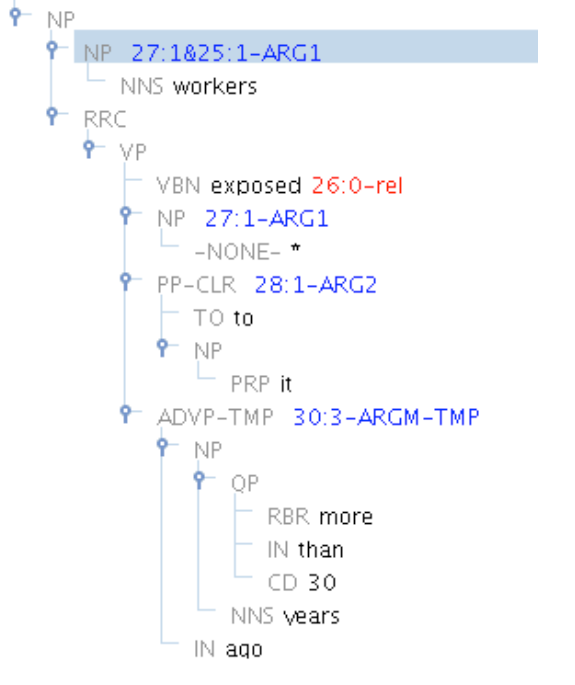
\includegraphics[scale=0.45]{img/redrelex.png}
\caption{\label{fig:redrelex}Пример размеченных данных \emph{PropBank}}
\end{figure}

Однако при использовании статистических моделей существует недостаток, который проявляется в зависимости от выбранного аннотированного ресурса. Кроме того, создание семантической разметки является трудозатратной и плохо формализуемой задачей. Из-за этого может проявляться некорректная работа на новых данных. Этот аспект принято называть проблемой доменной специфичности SRL.

%%%%%%%%%%%%%%%%%%%%%%%%%%%%%%%%%%%%%%%%%%%%%%%%
\subsection{Word Embeddings}

Статистические модели стали основным инструментом в задачах NLP, однако в начале они страдали от т.н. проклятия размерности \autocite{bellman1957dynamic}. Это повлекло развитие алгоритмов, которые позволили бы представлять слова в низкоразмерном пространстве.

Стоит сказать, что на данный момент нет общепризнанного перевода термина embedding (от англ. ‘вложение’), поэтому будет использоваться англицизм. 

Embedding представляет собой преобразование некой сущности в числовой вектор. Далее будут рассмотрены основные подходы, применяющиеся для решения данной задачи.

%%%%%%%%%%%%%%%%%%%%%%%%%%%%%%%%%%%%%%%%%%%%%%%%
\subsubsection{One-hot encoding}

Одним из первых решений задачи векторного представления слов был так называемый унитарный код. Он представлял собой вектор длины n, которая определяется количеством слов некоторого словаря, содержащий $n-1$ нулей и $1$ единицу. Индекс значащей единицы соответствовал расположению слова в данном словаре ---см. таблицу~\ref{tab:bow-ohe}.

\begin{table}
\centering
\caption{\label{tab:bow-ohe}One-Hot Encoded векторы}
\begin{tabular}{@{}lccccccccccc@{}}
\toprule
Vocabulary   & 1 & 2 & 3 & 4 & 5 & 6 & 7 & 8 & 9 & 10 \\ \midrule
bag          & 1 & 0 & 0 & 0 & 0 & 0 & 0 & 0 & 0 & 0  \\
words        & 0 & 1 & 0 & 0 & 0 & 0 & 0 & 0 & 0 & 0  \\
model        & 0 & 0 & 1 & 0 & 0 & 0 & 0 & 0 & 0 & 0  \\
way          & 0 & 0 & 0 & 1 & 0 & 0 & 0 & 0 & 0 & 0  \\
representing & 0 & 0 & 0 & 0 & 1 & 0 & 0 & 0 & 0 & 0  \\
text         & 0 & 0 & 0 & 0 & 0 & 1 & 0 & 0 & 0 & 0  \\
data         & 0 & 0 & 0 & 0 & 0 & 0 & 1 & 0 & 0 & 0  \\
simple       & 0 & 0 & 0 & 0 & 0 & 0 & 0 & 1 & 0 & 0  \\
understand   & 0 & 0 & 0 & 0 & 0 & 0 & 0 & 0 & 1 & 0  \\
implement    & 0 & 0 & 0 & 0 & 0 & 0 & 0 & 0 & 0 & 1  \\ \bottomrule
\end{tabular}
\end{table}

Несмотря на то, что такая архитектура позволяет решить проблему кодирования слов, она обладает рядом существенных недостатков:
\begin{itemize}
  \item При добавлении нового слова в середину существующего словаря есть необходимость заново проводить нумерацию его элементов.
  \item Происходит быстрый рост размерности представления текстов. \\ Например для текста из 9 уникальных слов требуется матрица 9х9
 \item Данный метод не предоставляет информации о семантической близости слов. Данный аспект связан с тем, что написание слов не имеет непосредственной связи с объектами, которые они описывают \autocite{saussure1916course}.
\end{itemize}

%%%%%%%%%%%%%%%%%%%%%%%%%%%%%%%%%%%%%%%%%%%%%%%%
\subsubsection{Bag of Words}
На основе кодирования слов унитарным кодом, рассмотренным в пункте 1.1.1, был предложен более экономичный вариант представления текстов, называемый “мешком слов” (от англ. Bag of words).

Алгоритм построения такого представления содержит следующие основные этапы:
\begin{itemize}
  \item Предварительное создание словаря методом OHE.
  \item Кодирование слов, содержащихся в тексте.
 \item Сложение всех полученных one-hot векторов.
\end{itemize}

На выходе получим числовой вектор, который описывает информацию о количестве различных слов в исходном тексте.
Такая модель не сохраняет структуру входных данных, в связи с чем теряется информация о взаимном расположении слов.
Тем не менее, применяя данный подход можно сравнивать тексты путем сравнения выходных векторов. Примером такой метрики является косинусная мера:

\begin{equation}\label{eq:cos}
{\displaystyle {\text{similarity}}=\cos(\theta )={\mathbf {A} \cdot \mathbf {B}  \over \|\mathbf {A} \|\|\mathbf {B} \|}={\frac {\sum \limits _{i=1}^{n}{A_{i}B_{i}}}{{\sqrt {\sum \limits _{i=1}^{n}{A_{i}^{2}}}}{\sqrt {\sum \limits _{i=1}^{n}{B_{i}^{2}}}}}},}
\end{equation}

$A_{i}$, $B_{i}$ -- компоненты векторов $\mathbf {A} $ и $ \mathbf {B}$ соответственно.\\

\begin{table}
\centering
\caption{\label{tab:bow-bow}Терм-документная таблица}
\begin{tabular}{@{}lcc@{}}
\toprule
Vocabulary   & \multicolumn{2}{l}{Documents} \\ \midrule
             	    & C1            & C2            \\ \midrule
bag          	    & 1               & 1             \\
words           & 1               & 1             \\
model           & 1               & 1             \\
way              & 1               & 0             \\
representing& 1               & 0             \\
text              & 1               & 0             \\
data             & 1               & 0             \\
simple           & 0               & 1             \\
understand   & 0               & 1             \\
implement    & 0               & 1             \\ \bottomrule
\end{tabular}
\end{table}

Рассмотрим этот процесс имплементации алгоритма.
\begin{enumerate}

  \item Зададим экземпляры текста.\\C1 = \textit{“The Bag of Words model is a way of representing text data.”}\\
	C2 = \textit{“The Bag of Words model is simple to understand and implement.”}
  \item Очистим тексты от пунктуационных символов и ‘стоп-слов’\footnote{the, of, is, a, to, and}, которые не несут смысловой нагрузки. 
   \item Сформируем словарь и закодируем его методом OHE (см. таблицу~\ref{tab:bow-ohe}).

  \item Для каждого предложения сложим One-Hot векторы слов, которые входят в их составы (см. таблицу~\ref{tab:bow-bow}). 
  
  \item Применим косинусную меру \eqref{eq:cos} к полученным векторам, которые количественно описывают исходные тексты.
\begin{equation*}
{\displaystyle {\text{similarity}}=\cos(\theta )= \frac{3} { \sqrt{7} \cdot  \sqrt{6}}= {0.46291}}
\end{equation*}
\end{enumerate}
Кроме того, полученную Таблицу \ref{tab:bow-bow}  с зависимостью “слово-документ” можно представить в виде произведения матриц “слово-тема” и “тема-документ”. Для этого можно использовать SVD-разложение:

\begin{eqnarray}\label{eq:svd}
{\displaystyle 
{\begin{matrix}

\\&({\textbf {d}}_{j})&&&&&&&\\&\downarrow &&&&&&& \\({\textbf {t}}_{i}^{T})\rightarrow &{
\begin{bmatrix}x_{1,1}&\dots &x_{1,n}\\\\\vdots &\ddots &\vdots \\\\x_{m,1}&\dots &x_{m,n}\\\end{bmatrix}}&=
\\&= {\begin{bmatrix}
{\begin{bmatrix}\,\\\,\\{\textbf {u}}_{1}\\\,\\\,\end{bmatrix}}\dots  
{\begin{bmatrix}\,\\\,\\{\textbf {u}}_{l}\\\,\\\,\end{bmatrix}}
\end{bmatrix}}&\cdot &
   {\begin{bmatrix}\sigma _{1}&\dots &0\\\vdots &\ddots &\vdots \\0&\dots &\sigma _{l}\\\end{bmatrix}}&\cdot &
   {\begin{bmatrix}
   {\begin{bmatrix}&&{\textbf {v}}_{1}&&\end{bmatrix}}\\\vdots \\
   {\begin{bmatrix}&&{\textbf {v}}_{l}&& \end{bmatrix}}
   \end{bmatrix}}
 \end{matrix}}}
\end{eqnarray}

${\textbf {t}}_{i}$  -- слово, ${\textbf {d}}_{i}$ -- документ.\\

Применим такое разложение для текстов из примера и визуализируем (см.~рис.~\ref{fig:svd-example}).
Как можно видеть, получаемые результаты имеют сильную зависимость от корпуса, к которому применяется разложение.

%%%%%%%%%%%%%%%%
\begin{figure}[h]
\centering
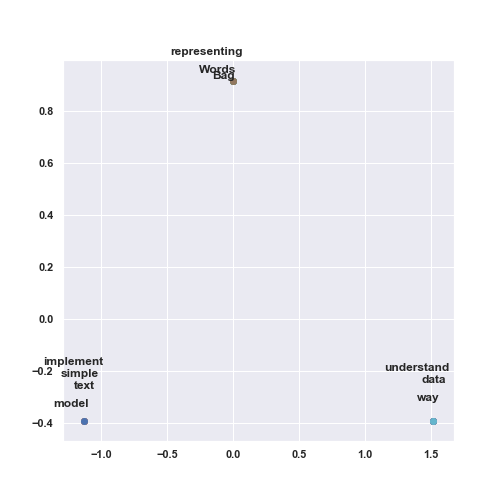
\includegraphics[width=0.65\textwidth]{img/svd-example.png}
\caption{\label{fig:svd-example}SVD разложение для C1 и С2}
\end{figure}
%%%%%%%%%%%%%%%%

%%%%%%%%%%%%%%%%%%%%%%%%%%%%%%%%%%%%%%%%%%%%%%%%
\subsubsection{Word2vec}

Из-за ряда недостатков, которыми обладали традиционные алгоритмы, исследования в области представлений слов продолжились. В 2013 году Томаш Миколов представил подход \autocite{DBLP:journals/corr/abs-1301-3781} к кодированию слов, который решал целый ряд проблем, присущих другим моделям, в том числе рост размерности векторного пространства и невозможность сохранять семантическую близость.

Им было представлено 2 подхода, которые он назвал continuous bag-of-words (CBOW) и skip-gram. Они позволяют строить высококачественные распределенные векторные представлений.

Между представленными моделями есть существенное отличие. CBOW вычисляет условную вероятность появления целевого слова исходя из его контекста,  который лежит в окне размера $k$. В свою очередь skip-gram предсказывает слова контекста по центральному слову. Предполагается, что контекстные слова расположены симметрично целевым словам на расстоянии, равном размеру окна в обоих направлениях. Схематичное представление данных методов показано на ~рис.~\ref{fig:w2v-models}

%%%%%%%%%%%%%%%%
\begin{figure}[t]
\centering
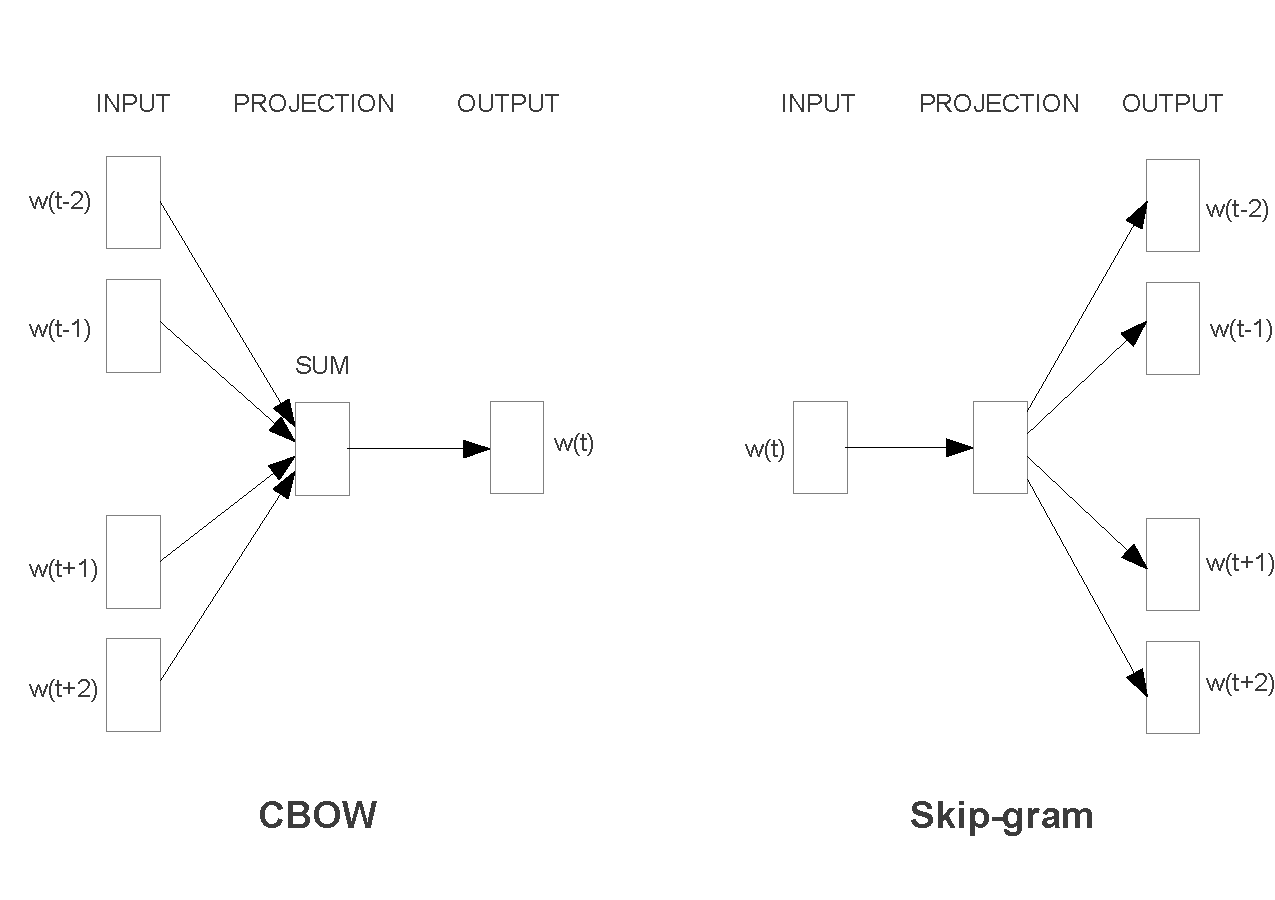
\includegraphics[width=0.7\textwidth]{img/efficient-models}
\caption{\label{fig:w2v-models}Модели CBOW и Skip-gram (Источник рисунка: \hspace{\textwidth}Mikolov \autocite{DBLP:journals/corr/abs-1301-3781})}
\end{figure}
%%%%%%%%%%%%%%%%

\paragraph{Модель CBOW} Рассмотрим упрощенную модель CBOW (см.~рис.~\ref{fig:w2v-cbow}) с контекстом из одного слова более детально. Она представляет собой полносвязную нейронную сеть со скрытым слоем. Входной слой, принимающий one-hot вектор, состоит из ${V}$ нейронов, а скрытый слой из ${N}$ нейронов. На выходном слое применяется операция Softmax, давая на выходе распределение вероятностей по всем словам в словаре. Слои связаны матрицами весов ${\textbf W} \in \mathcal{R}^{V \times N } $ и ${\textbf W^{'}} \in \mathcal{R}^{N \times V}$ соответственно.

\begin{figure}[ht]
\centering
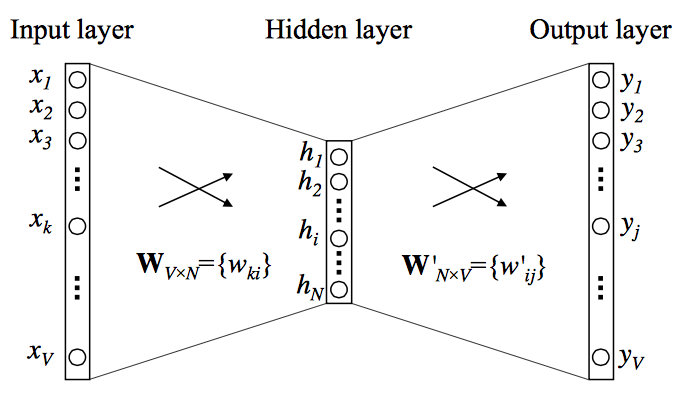
\includegraphics[width=0.7\textwidth]{img/CBOW.png}
\caption{\label{fig:w2v-cbow}Модель CBOW (Источник рисунка: Rong~\autocite{Rong2014word2vecPL})}
\end{figure}


Каждая строка матрицы ${\textbf W}$ это $N$-мерное векторное представление $\mathbf{v}_w$ связанного слова входного слоя. Формально можно записать строку $i$ матрицы $\textbf{W}$ как $\mathbf{v}_w^T$.

Таким образом, 
\begin{equation}
\mathbf{h} = \mathbf{W}^T \mathbf{x} = \mathbf{W}_{(k, \cdot)}^T := \mathbf{v}_{w_I}^T,
\label{eq:cbow-h}
\end{equation}
где $\mathbf{v}_{w_I}$ - векторное представление входного слова $\mathbf{w_I}$.

Скрытый и выходной слой связаны матрицей $\mathbf{W}' = \{w'_{ij}\}$. Используя данную матрицу весов можно посчитать оценку $u_j$ для каждого слова из словаря
\begin{equation}
u_j = {\mathbf{v}'_{w_j}}^T \mathbf{h},
\label{eq:cbow-uj}
\end{equation}
где  $\mathbf{v}'_{w_j}$ это $j$-я колонка матрицы W'. После этого используется нелинейная функция Softmax (\ref{eq:cbow-yj}) для получения апостериорного распределения слов.
\begin{equation}
p(w_j | w_I) = y_j = \frac{\exp(u_j)}{\sum_{j'=1}^V\exp(u_{j'})},
\label{eq:cbow-yj}
\end{equation}
где $y_j$ является выходом $j$-го нейрона на выходном слое.
Используя формулы (\ref{eq:cbow-h}) и (\ref{eq:cbow-uj}) можно записать (\ref{eq:cbow-yj}) в следующем виде:
\begin{equation}
p(w_j | w_I) = \frac{\exp\left({\mathbf{v}'_{w_j}}^T\mathbf{v}_{w_I}\right)}{\sum_{j'=1}^V\exp\left({\mathbf{v}'_{w_{j'}}}^T\mathbf{v}_{w_I}\right)}
\label{eq:cbow-pwo}
\end{equation}

Учитывая,  что $\mathbf{v}_w$ и $\mathbf{v}'_w$ - представления слова w через строки матрицы $\mathbf{W}$ и колонки матрицы $\mathbf{W'}$ соответственно. Будем называть $\mathbf{v}_w$  «входным вектором», а $\mathbf{v}'_w$ - «выходным вектором» слова w. 

В качестве функции потерь, которую следует минимизировать, используется логарифмическая функция правдоподобия
\begin{equation}
E=-\log p(w_O|w_I)
\label{eq:cbow-loss}
\end{equation}
где $w_I$ - входное слово, а $w_O$- предсказанное.

\begin{figure}[t]
\centering
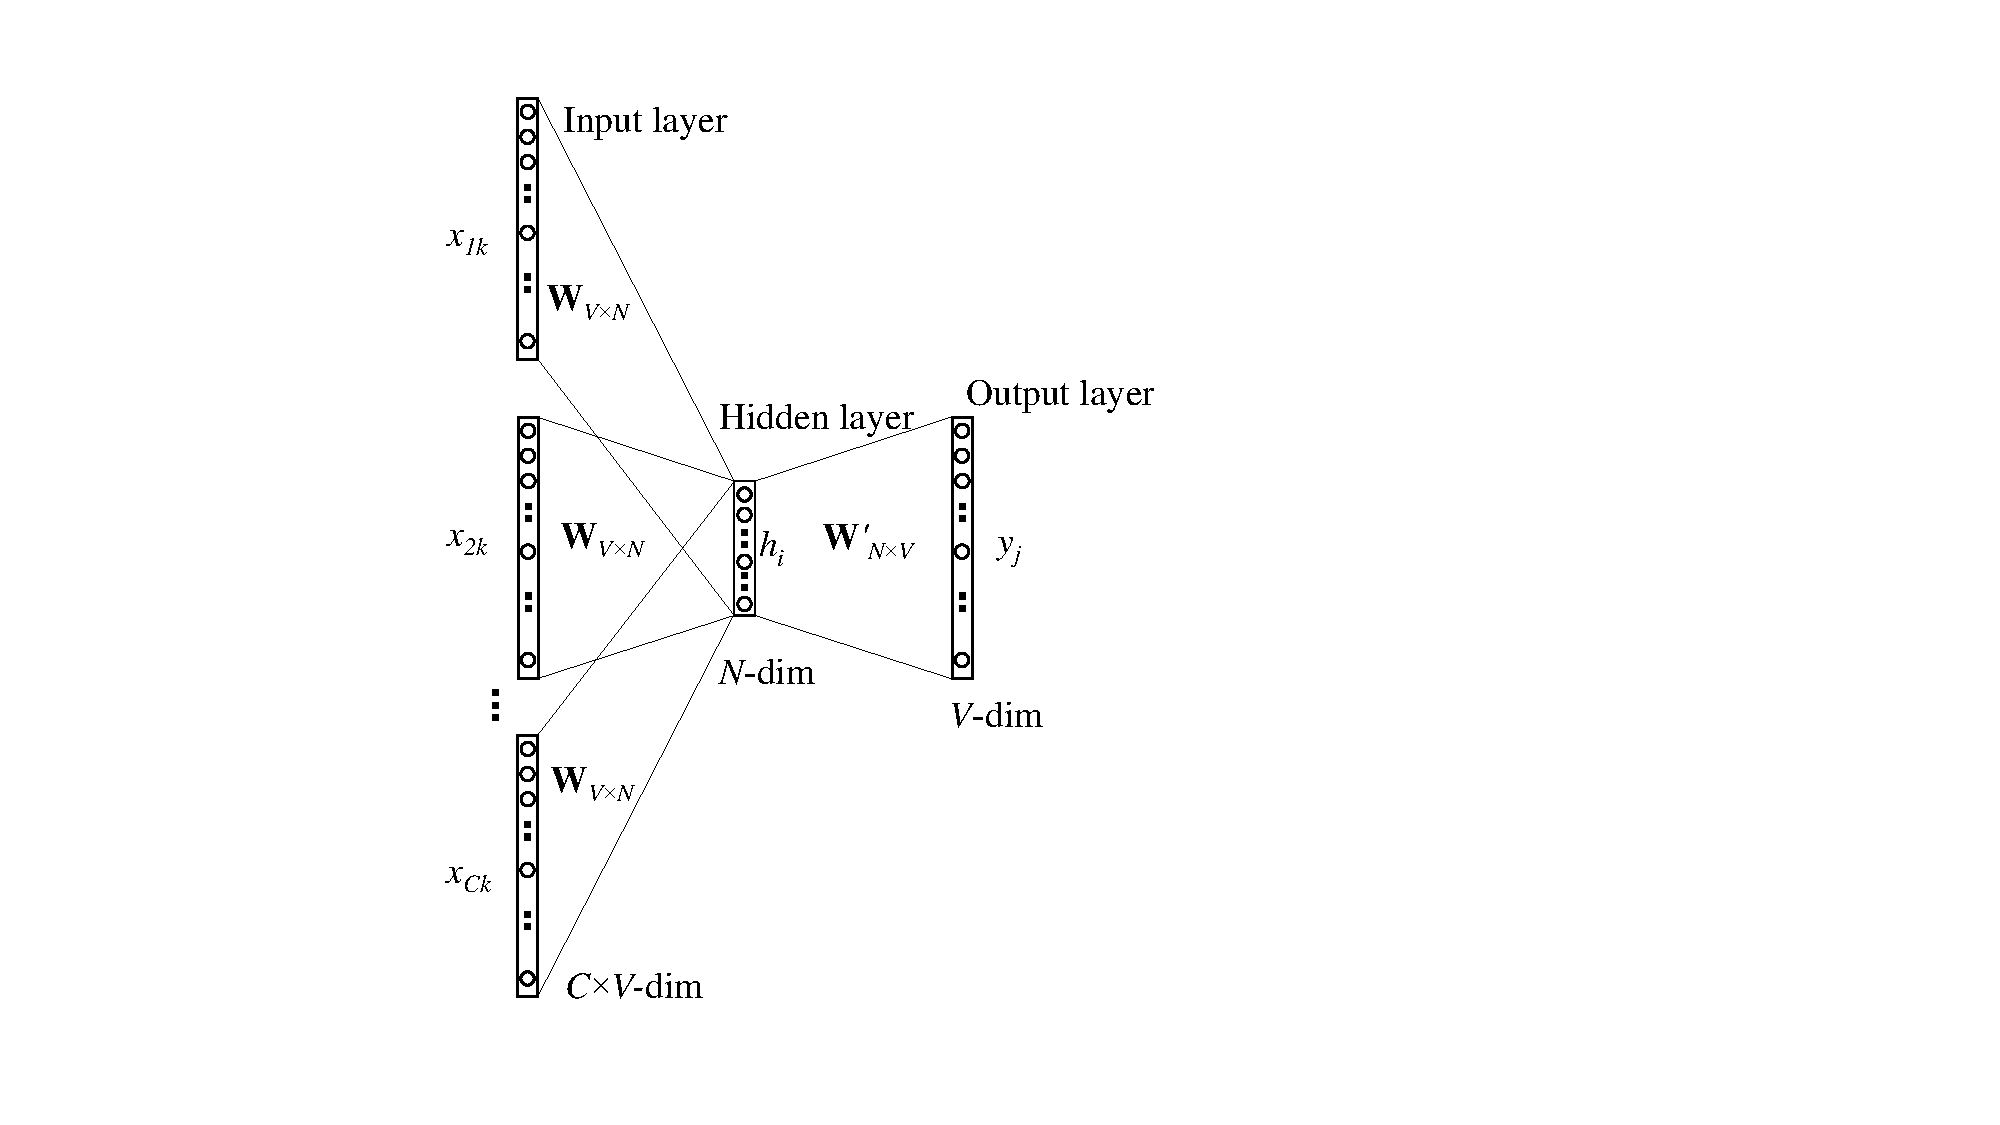
\includegraphics[width=0.42\textwidth]{img/cbow-multi.pdf}
\caption{\label{fig:cbow-multi} Модель CBOW в общем случае}
\end{figure}

В общем случае модели CBOW см.~рис.~\ref{fig:cbow-multi}, когда контекст превышает одно слово, при вычислении выходных значений скрытого слоя подсчитывается среднее значение векторов контекста:
\begin{eqnarray}
\mathbf{h} &=& \frac{1}{C}\mathbf{W}^T(\mathbf{x}_1+\mathbf{x}_2+\cdots+\mathbf{x}_C) \\
&=& \frac{1}{C}(\mathbf{v}_{w_1} + \mathbf{v}_{w_2} + \cdots + \mathbf{v}_{w_C})^T
\label{eq:cbow-complex-h}
\end{eqnarray}
где $C$- количество слов в контексте, $w_1, \cdots, w_C$ - контекстные слова, $\mathbf{v}_w$  - входное слово $w$.



\paragraph{Модель Skip-gram}

Рассматриваемая общая модель (см.~рис.~\ref{fig:skip-gram-multi}) является обратной к CBOW. Теперь целевое слово подается на входной слой, а предсказание контекстных слов является результатом работы модели. 

Будем использовать обозначение $\mathbf{v}_{w_I}$ для входного вектора. Через $\mathbf{h}$ обозначим выходные данные скрытого слоя, которые останутся прежними:
\begin{equation}
\mathbf{h} = \mathbf{W}_{(k, \cdot)}^T := \mathbf{v}_{w_I}^T,
\end{equation}

\begin{figure}[t]
\centering
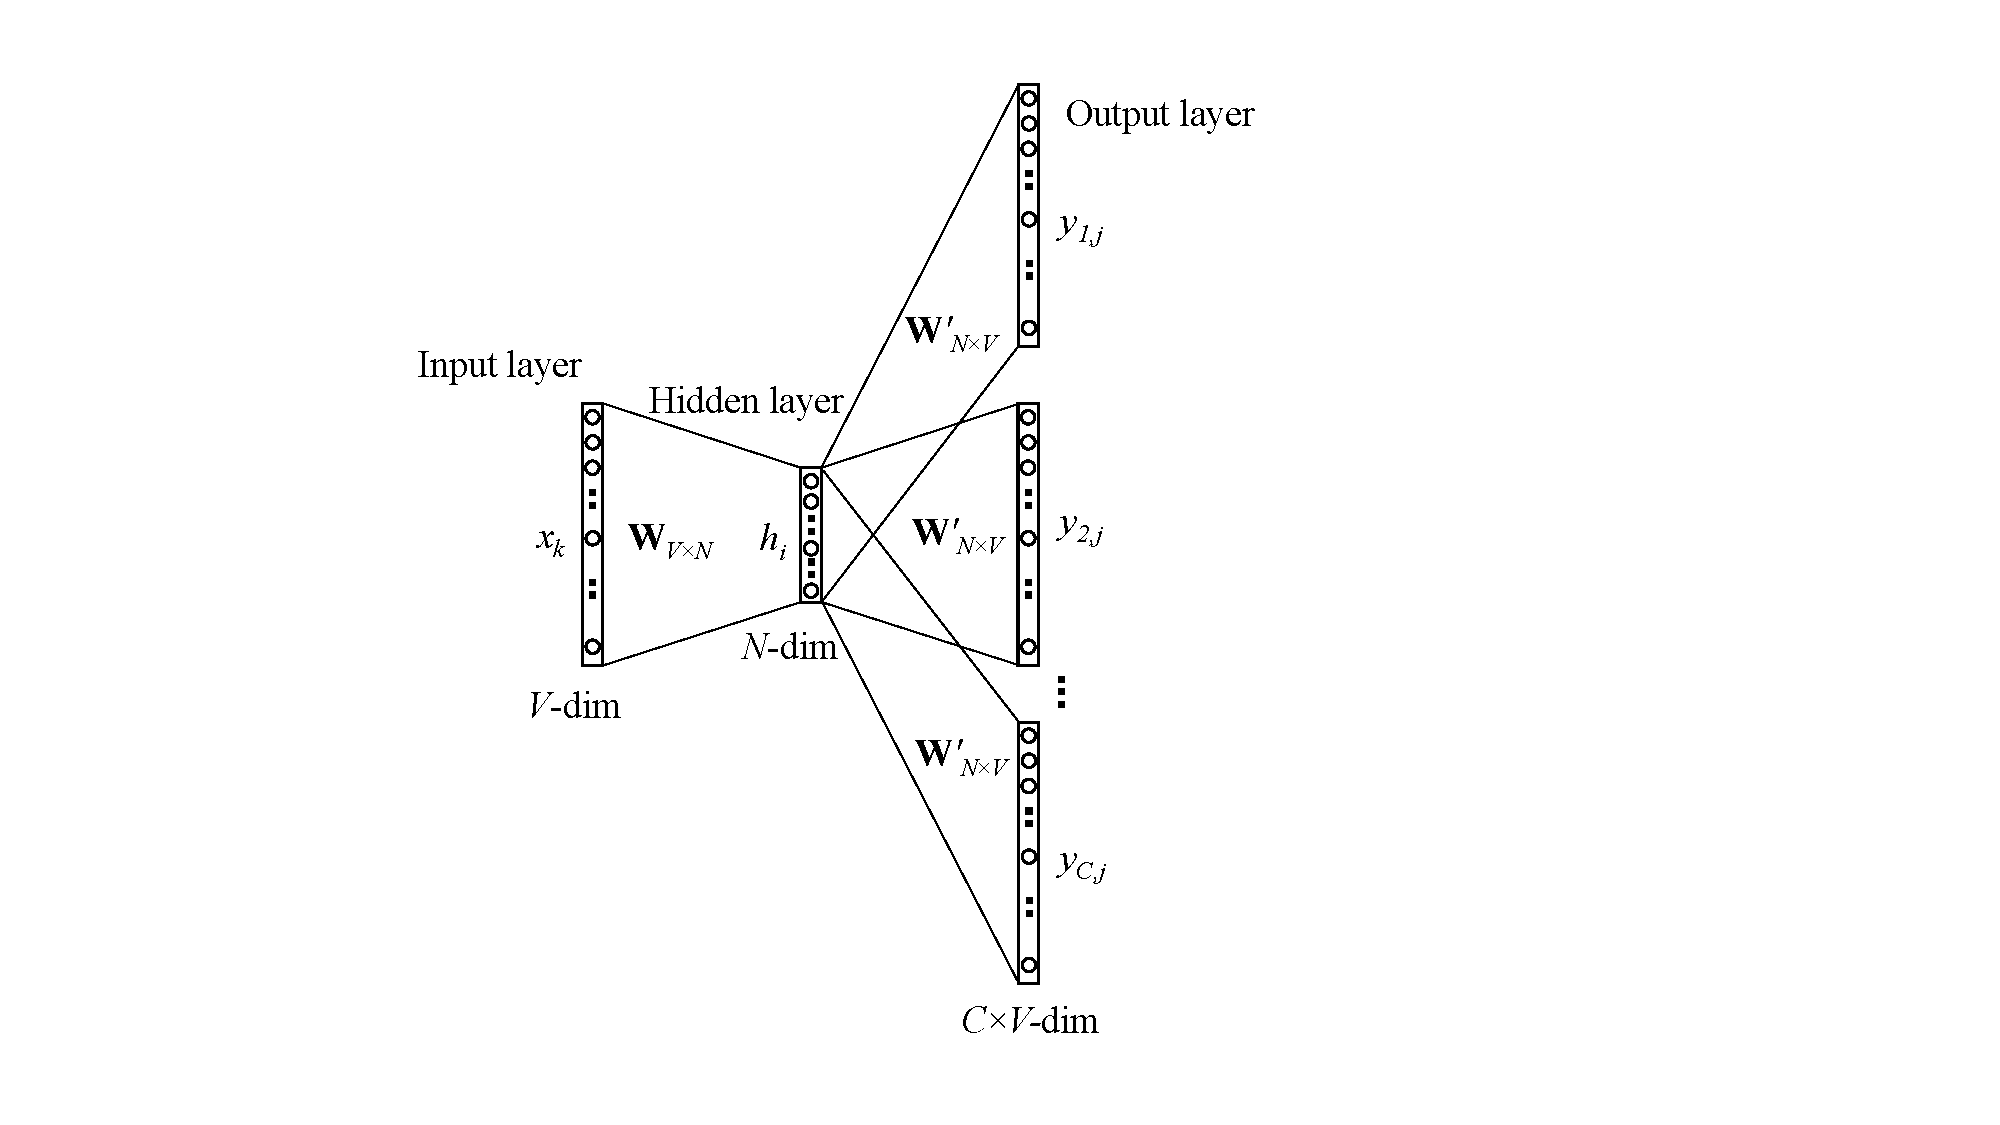
\includegraphics[width=0.42\textwidth]{img/skip-gram-multi.pdf}
\caption{\label{fig:skip-gram-multi} Модель Skip-gram в общем случае}
\end{figure}

Будем использовать обозначение  $\mathbf{v}_{w_I}$ для входного вектора. Через $\mathbf{h}$ обозначим выходные данные скрытого слоя:
\begin{equation}
\mathbf{h} = \mathbf{W}_{(k, \cdot)}^T := \mathbf{v}_{w_I}^T,
\end{equation}

Выходной же слой теперь формирует $C$ полиномиальных распределений вместо одного. Каждый элемент выходного слоя считается с использование матриц скрытого и выходного слоя.

\begin{equation}
p(w_{c,j} = w_{O,c} | w_I) = y_{c,j} = \frac{\exp(u_{c,j})}{\sum_{j'=1}^V\exp(u_{j'})}
\end{equation}
$w_{c,j}$ -- $j$-е слово в $c$-м векторе выходного слоя;\\
$w_{O,c}$  -- действительное $c$-е выходное контекстное слово; \\
$w_I$ -- единственное входное слово;\\
$y_{c,j}$ -- предсказание $j$-го элемента в $c$-м векторе выходного слоя;\\
$u_{c,j}$  -- входные данные $j$-го элемента в $c$-м векторе выходного слоя;\\


Функция потерь также меняется и принимает следующий вид:
\begin{eqnarray}
E &=& -\log p(w_{O,1}, w_{O,2}, \cdots, w_{O,C} | w_I) \\
&=& -\log \prod_{c=1}^C\frac{\exp(u_{c,j_c^*})}{\sum_{j'=1}^V\exp(u_{j'})} \\
&=& -\sum_{c=1}^C u_{j_c^*} + C\cdot\log\sum_{j'=1}^V\exp(u_{j'})
\end{eqnarray}
где  $j_c^*$ -- индекс верного $c$-го выходного слова в словаре.

Таким образом, преимущество использования модели Skip-gram перед CBOW в том, что при том же корпусе текстов получается больше экземпляров обучающей выборки, из-за чего повышается точность предсказаний модели.
\begin{figure}[t]% p означает, что нужно выделить для рисунка
% отдельную страницу; применяется для больших рисунков
\centering
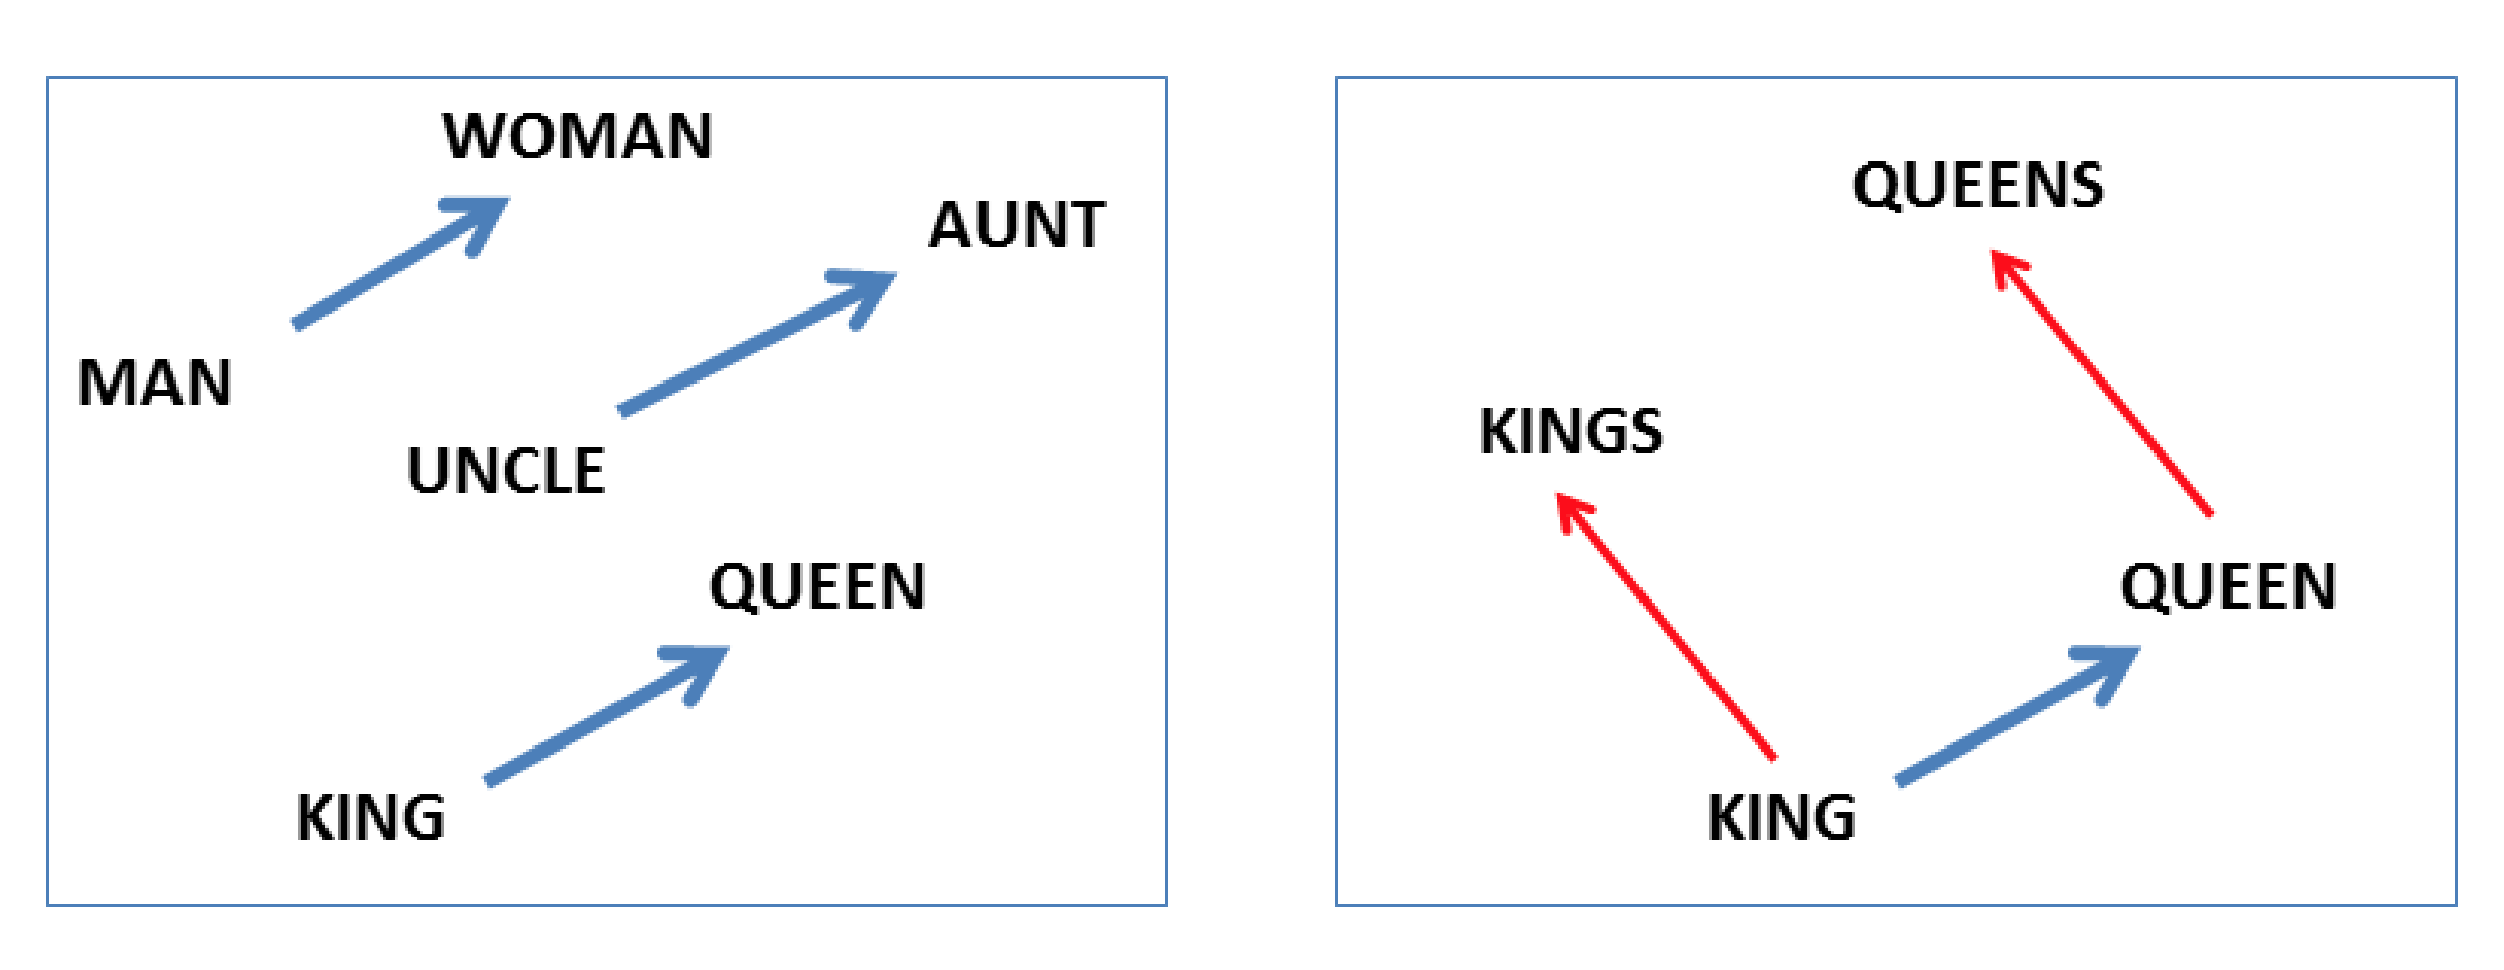
\includegraphics[width=0.7\textwidth]{img/w2v-semantic.png}
\caption{\label{fig:w2v-semantic}Иллюстрация отношений векторного представления слов (Источник рисунка: Mikolov~\autocite{mikolov-etal-2013-linguistic})}
\end{figure}
Резюмируя, модель word2vec позволяет решить основную проблему векторного представления слов- размерность выходных векторов. Кроме того необходимо отметить главную особенность таких архитектур, которая заключается в том, что несмотря на отсутствие сохранения порядка слов в контексте, так как входные векторы суммируются, они сохраняют некоторые семантические характеристики корпусов текста, на которых проводится обучение. В связи с этим схожие по смыслу слова имеют схожие векторные представления. Наиболее популярный пример сохранения семантической близости представлен на ~рис.~\ref{fig:w2v-semantic}.


\subsection{Применение CNN в задачах NLP}
\label{subsec:cnn}


Рассмотренный в предыдущем пункте метод векторного представления слов word2vec и схожие с ним (GloVe и др.) дали большой толчок в разработке архитектур глубоких нейронных сетей для задач NLP. Данные представления применяются  как первый слой обработки данных в deep learning моделях. 

Одним из методов извлечения признаков из текстовых данных является применение сверточных нейронных сетей (англ. Convolutional Neural Network, CNN).
В задачах NLP наиболее часто встречаются варианты мультизадачных моделей, в которых результаты работы низкоуровневых слоев служат входными данными (признаками) для более высокоуровневых. Так, например, корректные POS тэги слов помогают улучшить показатель точности на задачах построения дерева зависимости. 

Пример такой архитектуры был представлен авторами Коллобертом и Уэстоном \autocite{DBLP:journals/corr/abs-1103-0398}. В своей работе они использовать мультизадачную нейронную сеть, которая решает задачи определения частей речи, восстановления семантических ролей, поиск именованных сущностей и др. 

\begin{figure}[t]

\centering
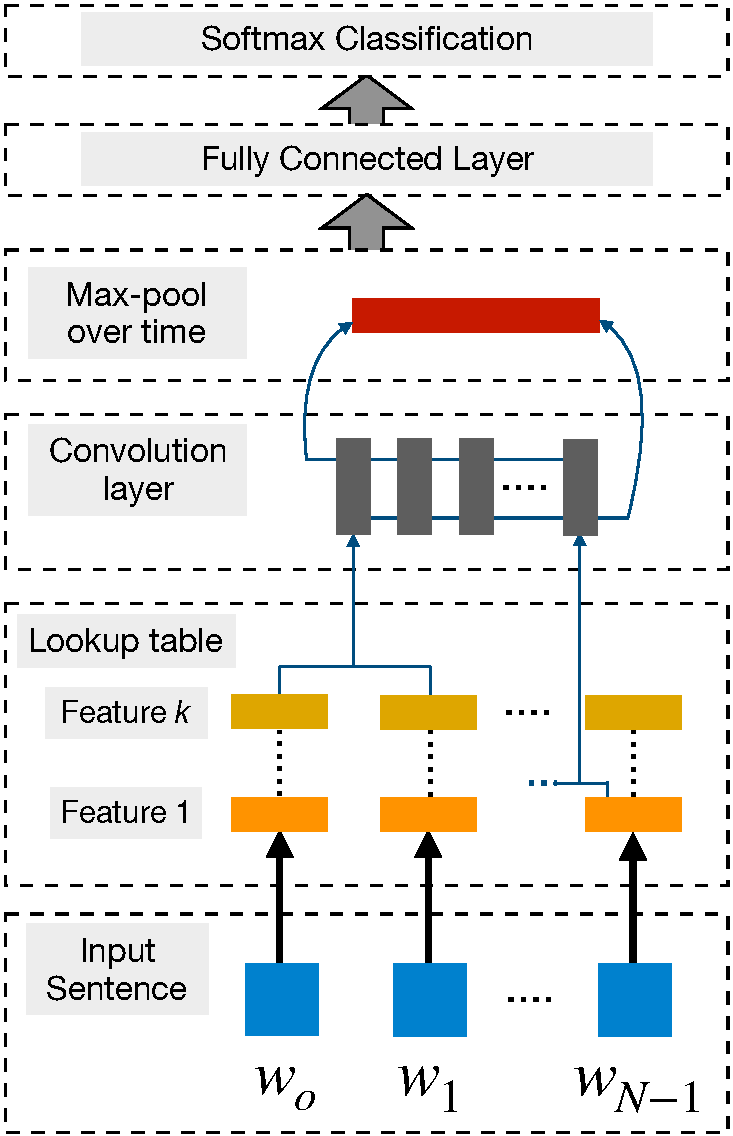
\includegraphics[width=0.45\textwidth]{img/collobertCNN.pdf}
\caption{\label{fig:collobertCNN}Пример CNN для задачи классификации на уровне слов\hspace{\textwidth}(Источник рисунка: Collobert~\autocite{10.1145/1390156.1390177})}
\end{figure}

Как видно из Рис.~\ref{fig:collobertCNN}, в этой архитектуре была использована таблица поиска (англ. lookup table) для векторного представления слов, благодаря которой последовательность слов $\{s_1, s_2, ... s_n\}$ была преобразована в некоторую последовательность векторов $\{ {{w}_{s_1}}, {{w}_{s_2}}, ... {{w}_{s_n}} \}$.

Сверточные нейронные сети способны извлекать информацию из n-грамм входного предложения, что дает возможность создания информативного семантического представления для последующих задач. Рассмотрим несколько архитектур и применений CNN для обработки естественного языка.

\subsubsection{Предсказание на уровне предложений}
\begin{figure}[t]
	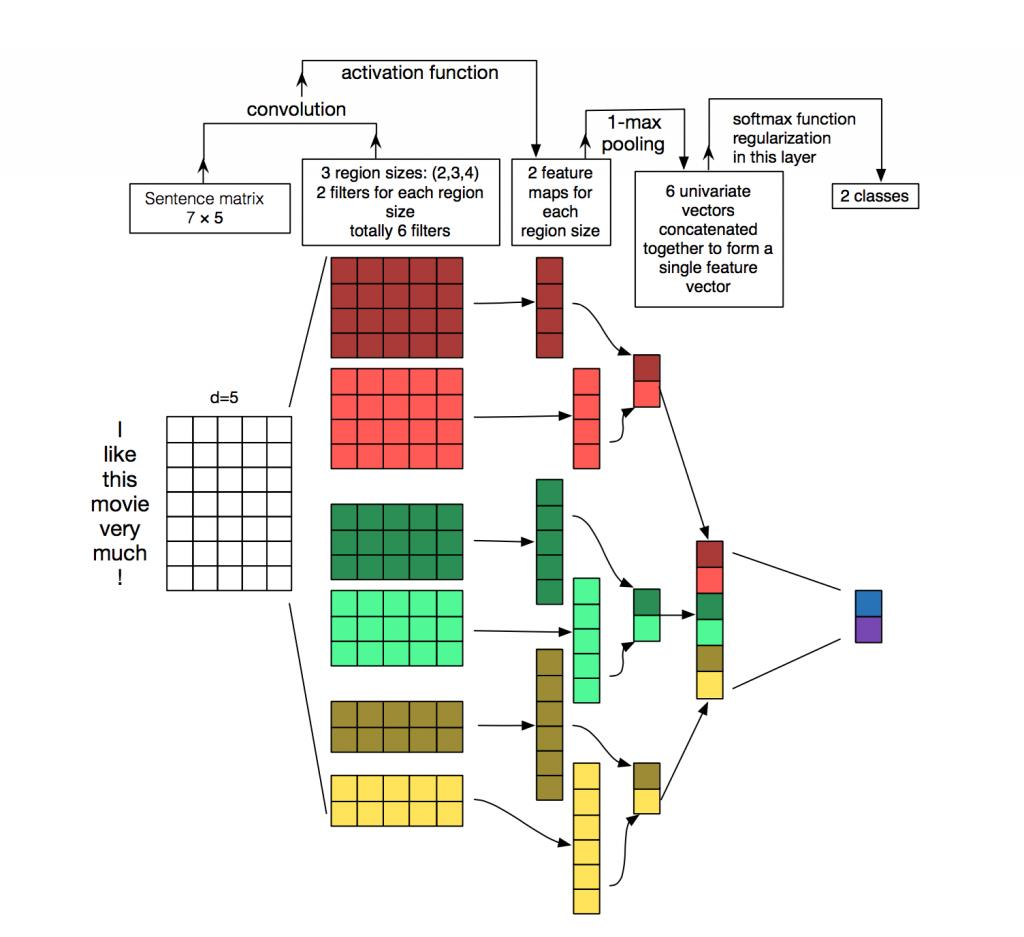
\includegraphics[scale=0.45]{img/CNN}
	\centering
	\caption{Модель CNN}\label{fig:CNN}
\end{figure}
Положим ${\mathbf w_{i}} \in \mathcal{R}^d$ - векторное представление $i$-го слова входного предложения, где $d$ - размерность векторов вложений. Тогда предложение, состоящее из n слов, может быть представлено матрицей вложений слов ${\mathbf W} \in \mathcal{R}^{n \times d}$. Пример такого представления можно увидеть на ~Рис.~\ref{fig:CNN}.

Обозначим ${\mathbf w_{i:i+j}} $ как конкатенацию векторов
 вложений слов ${\mathbf w_{i}}, {\mathbf w_{i+1}}, ... {\mathbf w_{i+j}}$. Начальная свертка применяется к этому входному слою и представляет собой фильтр ${\mathbf k} \in \mathcal{R}^{h \times d}$, который применяется к h словам, создавая новые признаки. Например, признак $c_i$ получается путем применения окна свертки к словам ${\mathbf w_{i:i+h-1}} $
\begin{equation}
c_i = f({\mathbf w_{i:i+h-1}}.{\mathbf k}^T + b )
\end{equation} 
 $b \in \mathcal{R}$ - смещение, $f$ - нелинейная функция активации (например, сигмоида). 
 
 Фильтр $k$ применяется ко всем возможным окнам текста и формирует карту признаков
\begin{equation}
c = [c_1, c_2, ... , c_{n-h+1}]
\end{equation} 

Стоит отметить, что представление текстовых данных отличается от представления изображений, к которым изначально применялись CNN. В отличие от них, текстовые данные представлены в двух, а не трех измерениях: ширине и количестве каналов. Ширину формирует количество слов в последовательности, а количество каналов - длина векторного представления слов. Учитывая то, что embedding слов сохраняет смысл только полностью, в задачах NLP применяются одномерные свертки (1D convolution), двигаясь только по оси, которая отвечает за количество слов.

\begin{figure}[t]
\centering
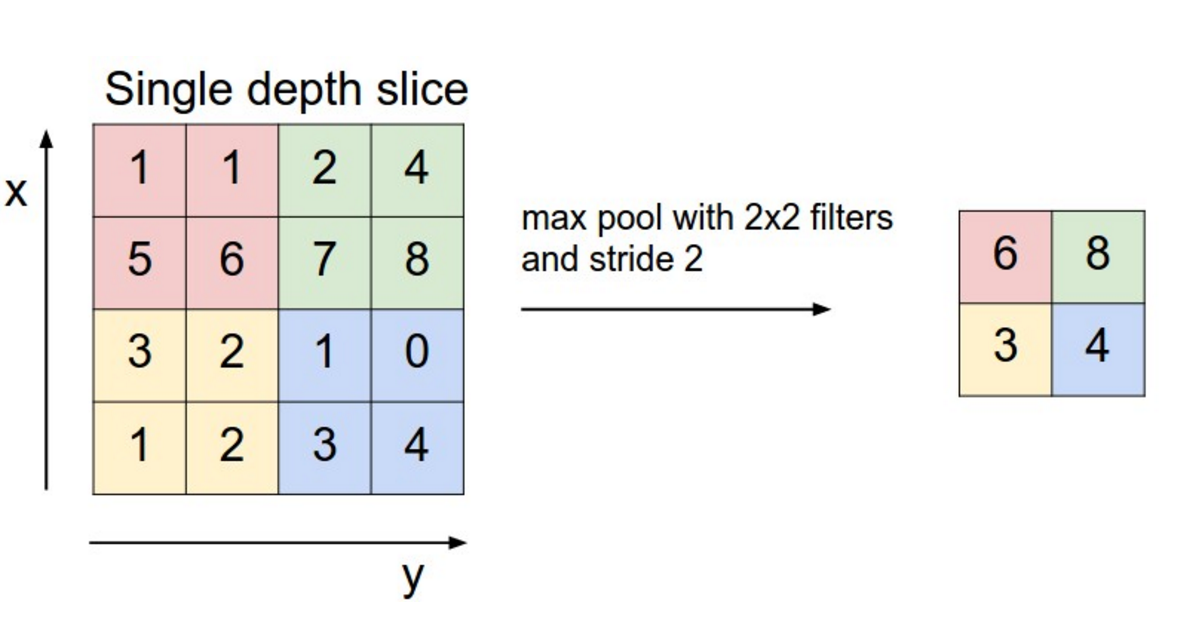
\includegraphics[width=0.8\textwidth]{img/maxpool}
\caption{\label{fig:maxpool}Операция \emph{max-pooling}}
\end{figure}

В CNN применяется множество фильтров различной ширины, что позволяет извлекать специфичную информацию из различных n-грамм. Чаще всего после сверточного слоя идет слой с операцией \emph{max-pooling}, которую обозначим $\hat{c} = max\{c\}$ (см.~рис.~\ref{fig:maxpool}). Эта операция выбирает максимальное значение из некоторого окна, проходясь по карте признаков. У применения такой операции есть несколько предпосылок.
Первая  -  \emph{max-pooling} обеспечивает контроль размерности выходных данных, что необходимо для задач классификации. Вторая причина заключается в том, что операция  \emph{max-pooling} позволяет более высокоуровневым слоям работать с информацией, которая захватывает больший участок данных, при этом такая операция передает наиболее значимые данные, полученные на всем предложении. 

Комбинации слоев свертки и \emph{max-pooling} выступают основными составляющими сверточной нейронной сети. Их последовательное применение совместно с большим количеством ядер свертки помогают улучшить качество анализа предложения и создавать абстрактные представления, содержащие семантическую информацию. При этом операции свертки на более глубоких слоях захватывают большую часть предложения. Такие операции продолжаются до тех пор, пока не захватят все предложение и не создадут обобщение его характеристик.

\subsubsection{Предсказание на уровне слов}
\begin{figure}[t]
\centering
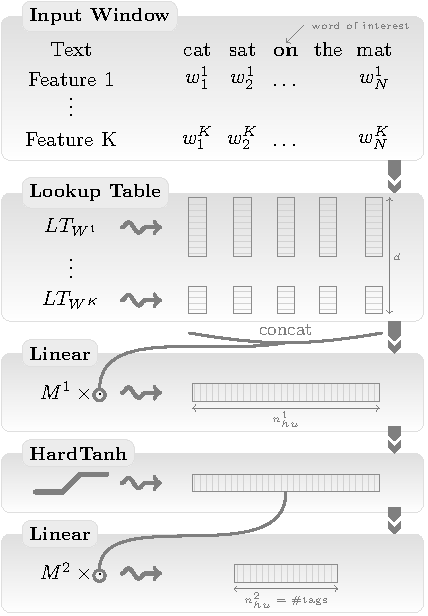
\includegraphics[width=0.4\textwidth]{img/network-window}
\caption{\label{fig:network-window}Модель Window Approach (Источник рисунка: \hspace{\textwidth}~Collobert \autocite{DBLP:journals/corr/abs-1103-0398})}
\end{figure}

Рассмотренная архитектура позволяет делать предсказания на уровне предложений, однако такой подход не решает ряд задач, в том числе описанных в пункте \ref{subsec:standard}. Для них необходимо производить предсказания на уровне слов. Адаптация CNN под такие задачи заключается в применении т.н. "оконного подхода" (англ. Window Approach).  Он основывается на гипотезе, что классификация слова зависит в первую очередь от слов, которые его окружают.

Таким образом, к каждому слову применяется окно фиксированного размера $2n + 1$, где целевое слово располагается в центре. Выделенный фрагмент теста рассматривается как под-предложение. Далее к нему применяется многослойная нейронная сеть и производится предсказание некоторых признаков целевого слова. Общая архитектура такой сети представлена на Рис.~\ref{fig:network-window}. Следует отметить, что она рассматривает слова как последовательности, что особенно актуально для таких задач, как SRL. 




% Please add the following required packages to your document preamble:
% \usepackage{booktabs}
% Please add the following required packages to your document preamble:
% \usepackage{booktabs}
\newpage
\section{Задача автоматического формирования заданий по грамматике}
Прикладная часть исследования заключается в создании системы, способной автоматически создавать задания по грамматике английского языка, используя в качестве входных данных произвольный текст. В качестве приоритетных направлений были выбраны задания вида Controlled Practice в разделах Active и Passive Voice с учетом всех возможных времен. 

Цель создания такой системы состоит в том, чтобы предоставить альтернативу стандартным учебникам и тренажерам по грамматике, которые используют заранее сформированные материалы и не дают достаточной гибкости в выборе методических материалов, что сказывается на заинтересованности студента в их изучении. 

В отличие от такого подхода, формирование заданий из пользовательских материалов может повысить вовлеченность и учесть специфическую лексику, которая используется в сферах, интересных конкретному пользователю.

Система представляет собой клиент-серверное приложение и состоит из 3х основных блоков:
\begin{itemize}
  \item получение и предобработка текстовых данных;
  \item поиск грамматических конструкций;
  \item визуализация результатов и обработка вводимых пользователем данных.
\end{itemize}

\subsection{Механика взаимодействия с пользователем}
Для взаимодействия с пользователем была выбрана концепция web-приложения, которое встраивается в браузер Chrome. Таким образом, для пользователя приложение представлено двумя элементами: расширением для браузера и web-страницей, на которой происходит визуализация результатов. 

В расширении предлагается выбрать основной раздел с заданиями, после чего конкретизировать свой запрос (см.~рис.~\ref{fig:ext}). 
\begin{figure}[h]
\centering
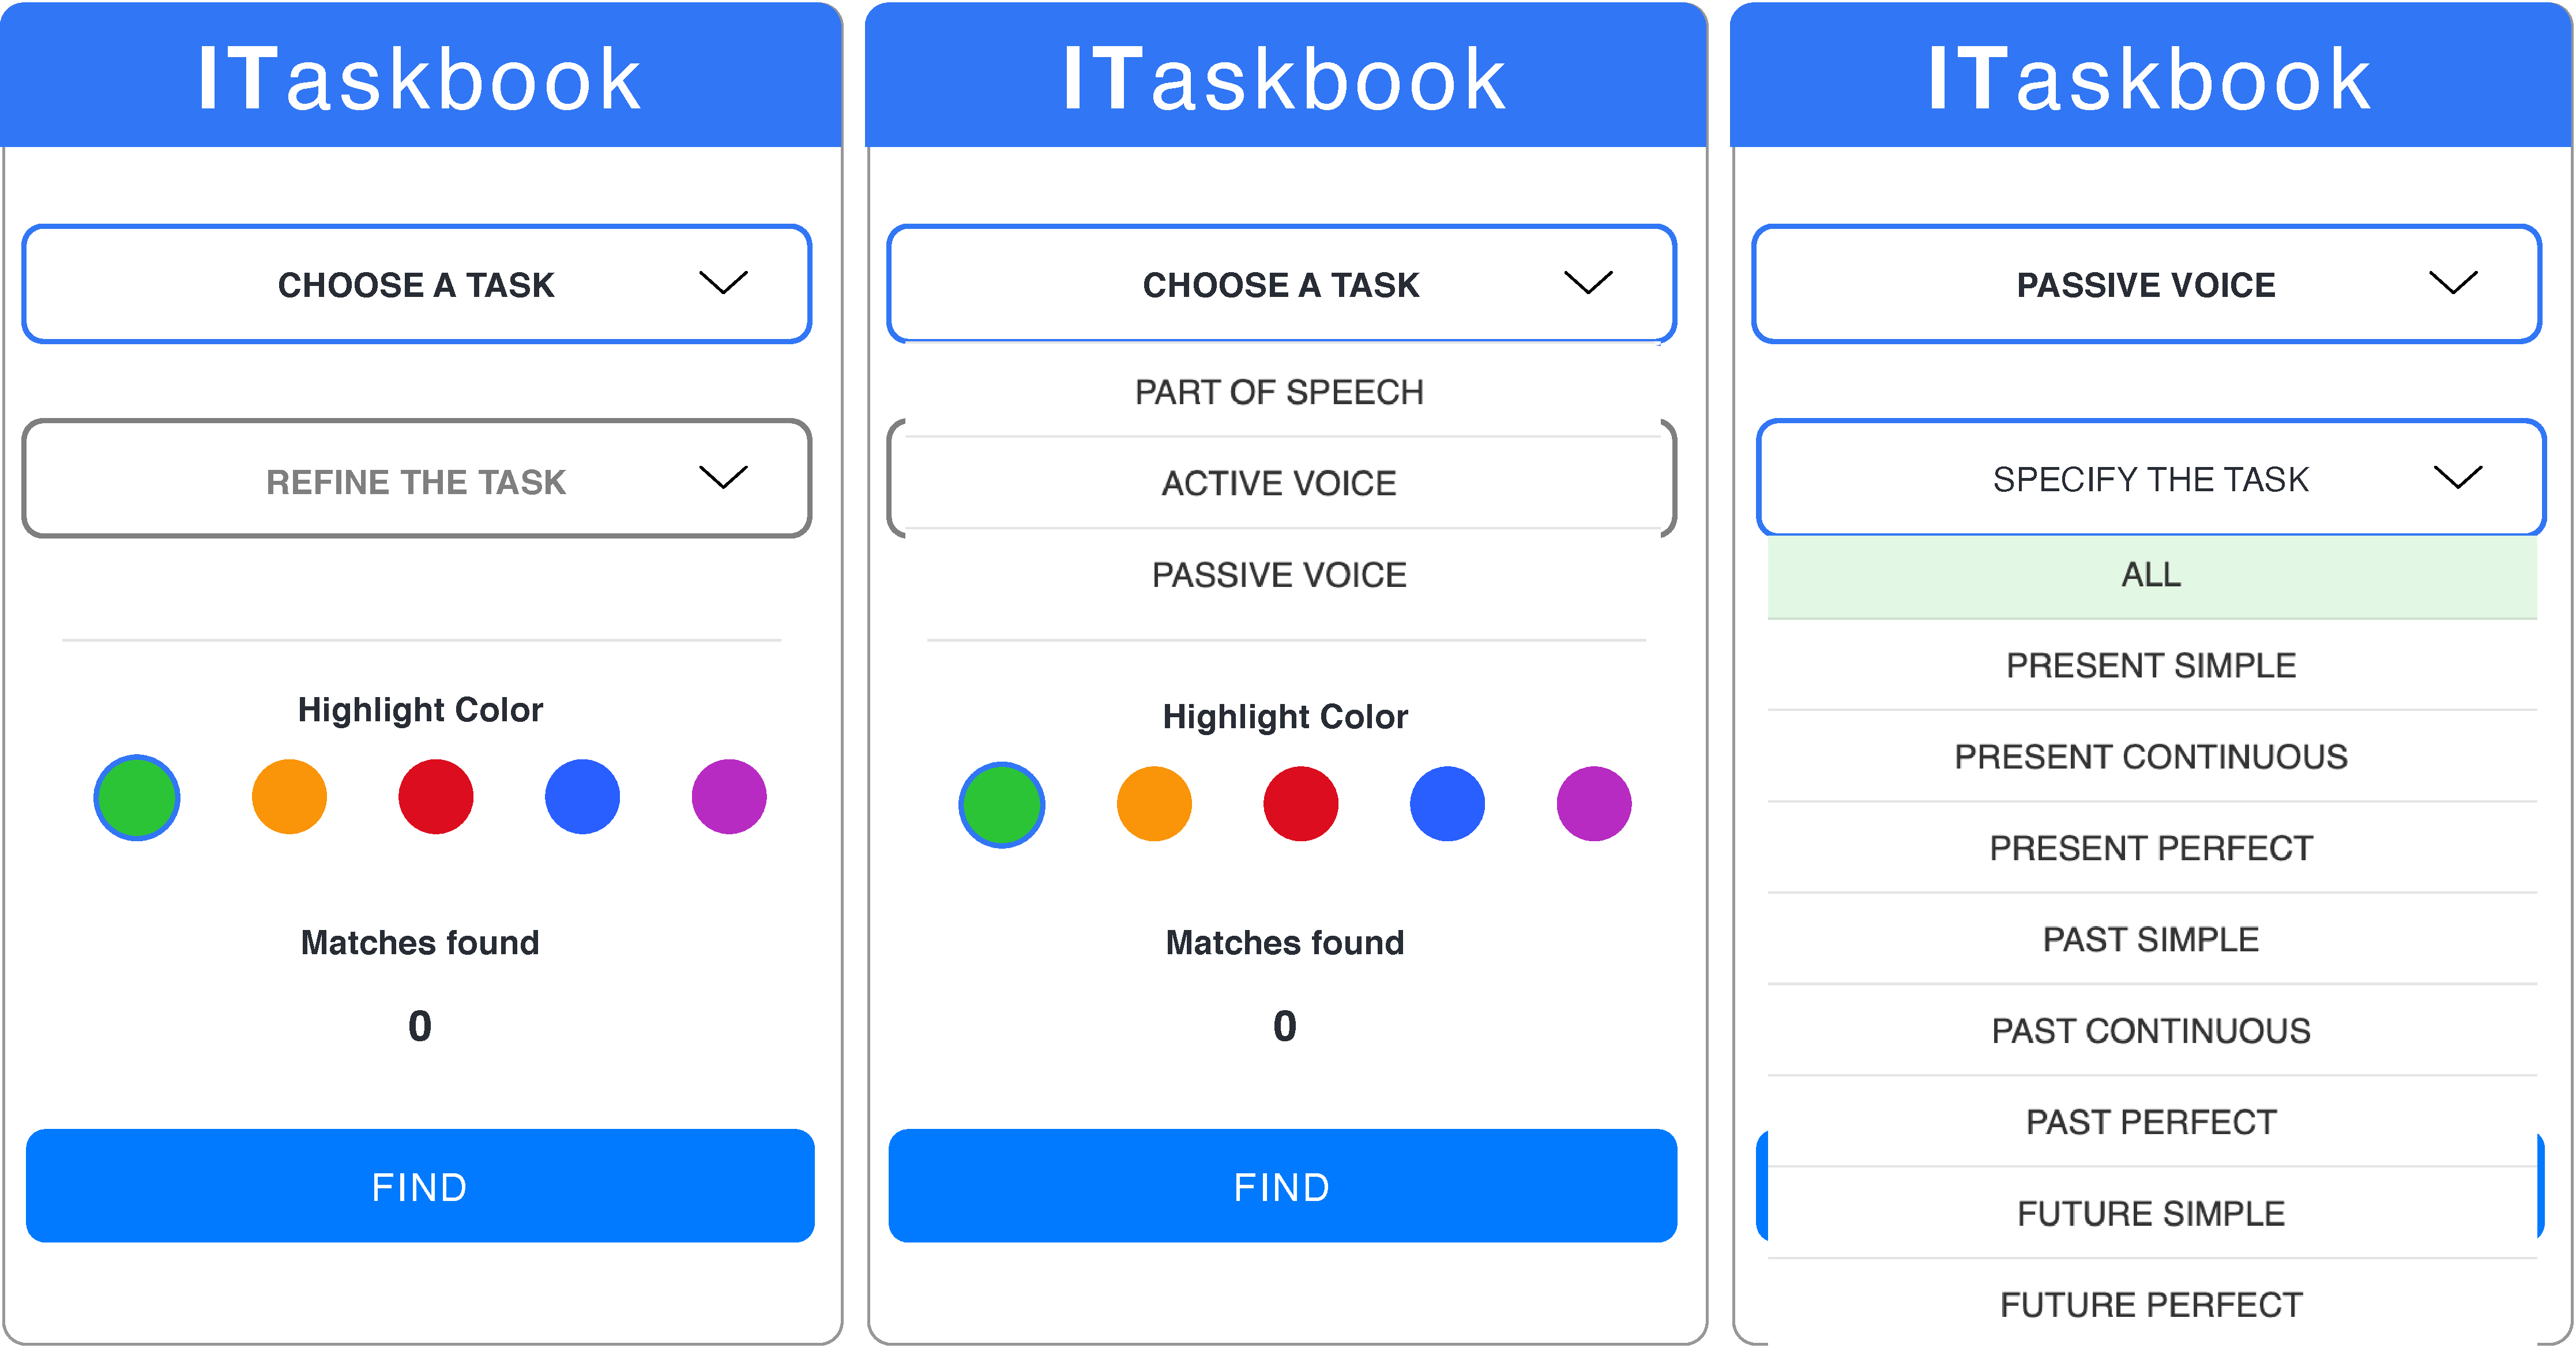
\includegraphics[width=0.3\textwidth]{img/ext}
\caption{\label{fig:ext}Расширение для браузера Chrome}
\end{figure}

На странице с заданиями, которые соответствуют запросу и  формируются на базе текстовой информации, находящейся на странице, где было вызвано расширение, пользователь может видеть свои результаты в интерактивном режиме (см.~рис.~\ref{fig:tasks-example}), при этом вся статистика ответов записывается и хранится как локально, так и на сервере в базе данных.
\begin{figure}[p]
\centering
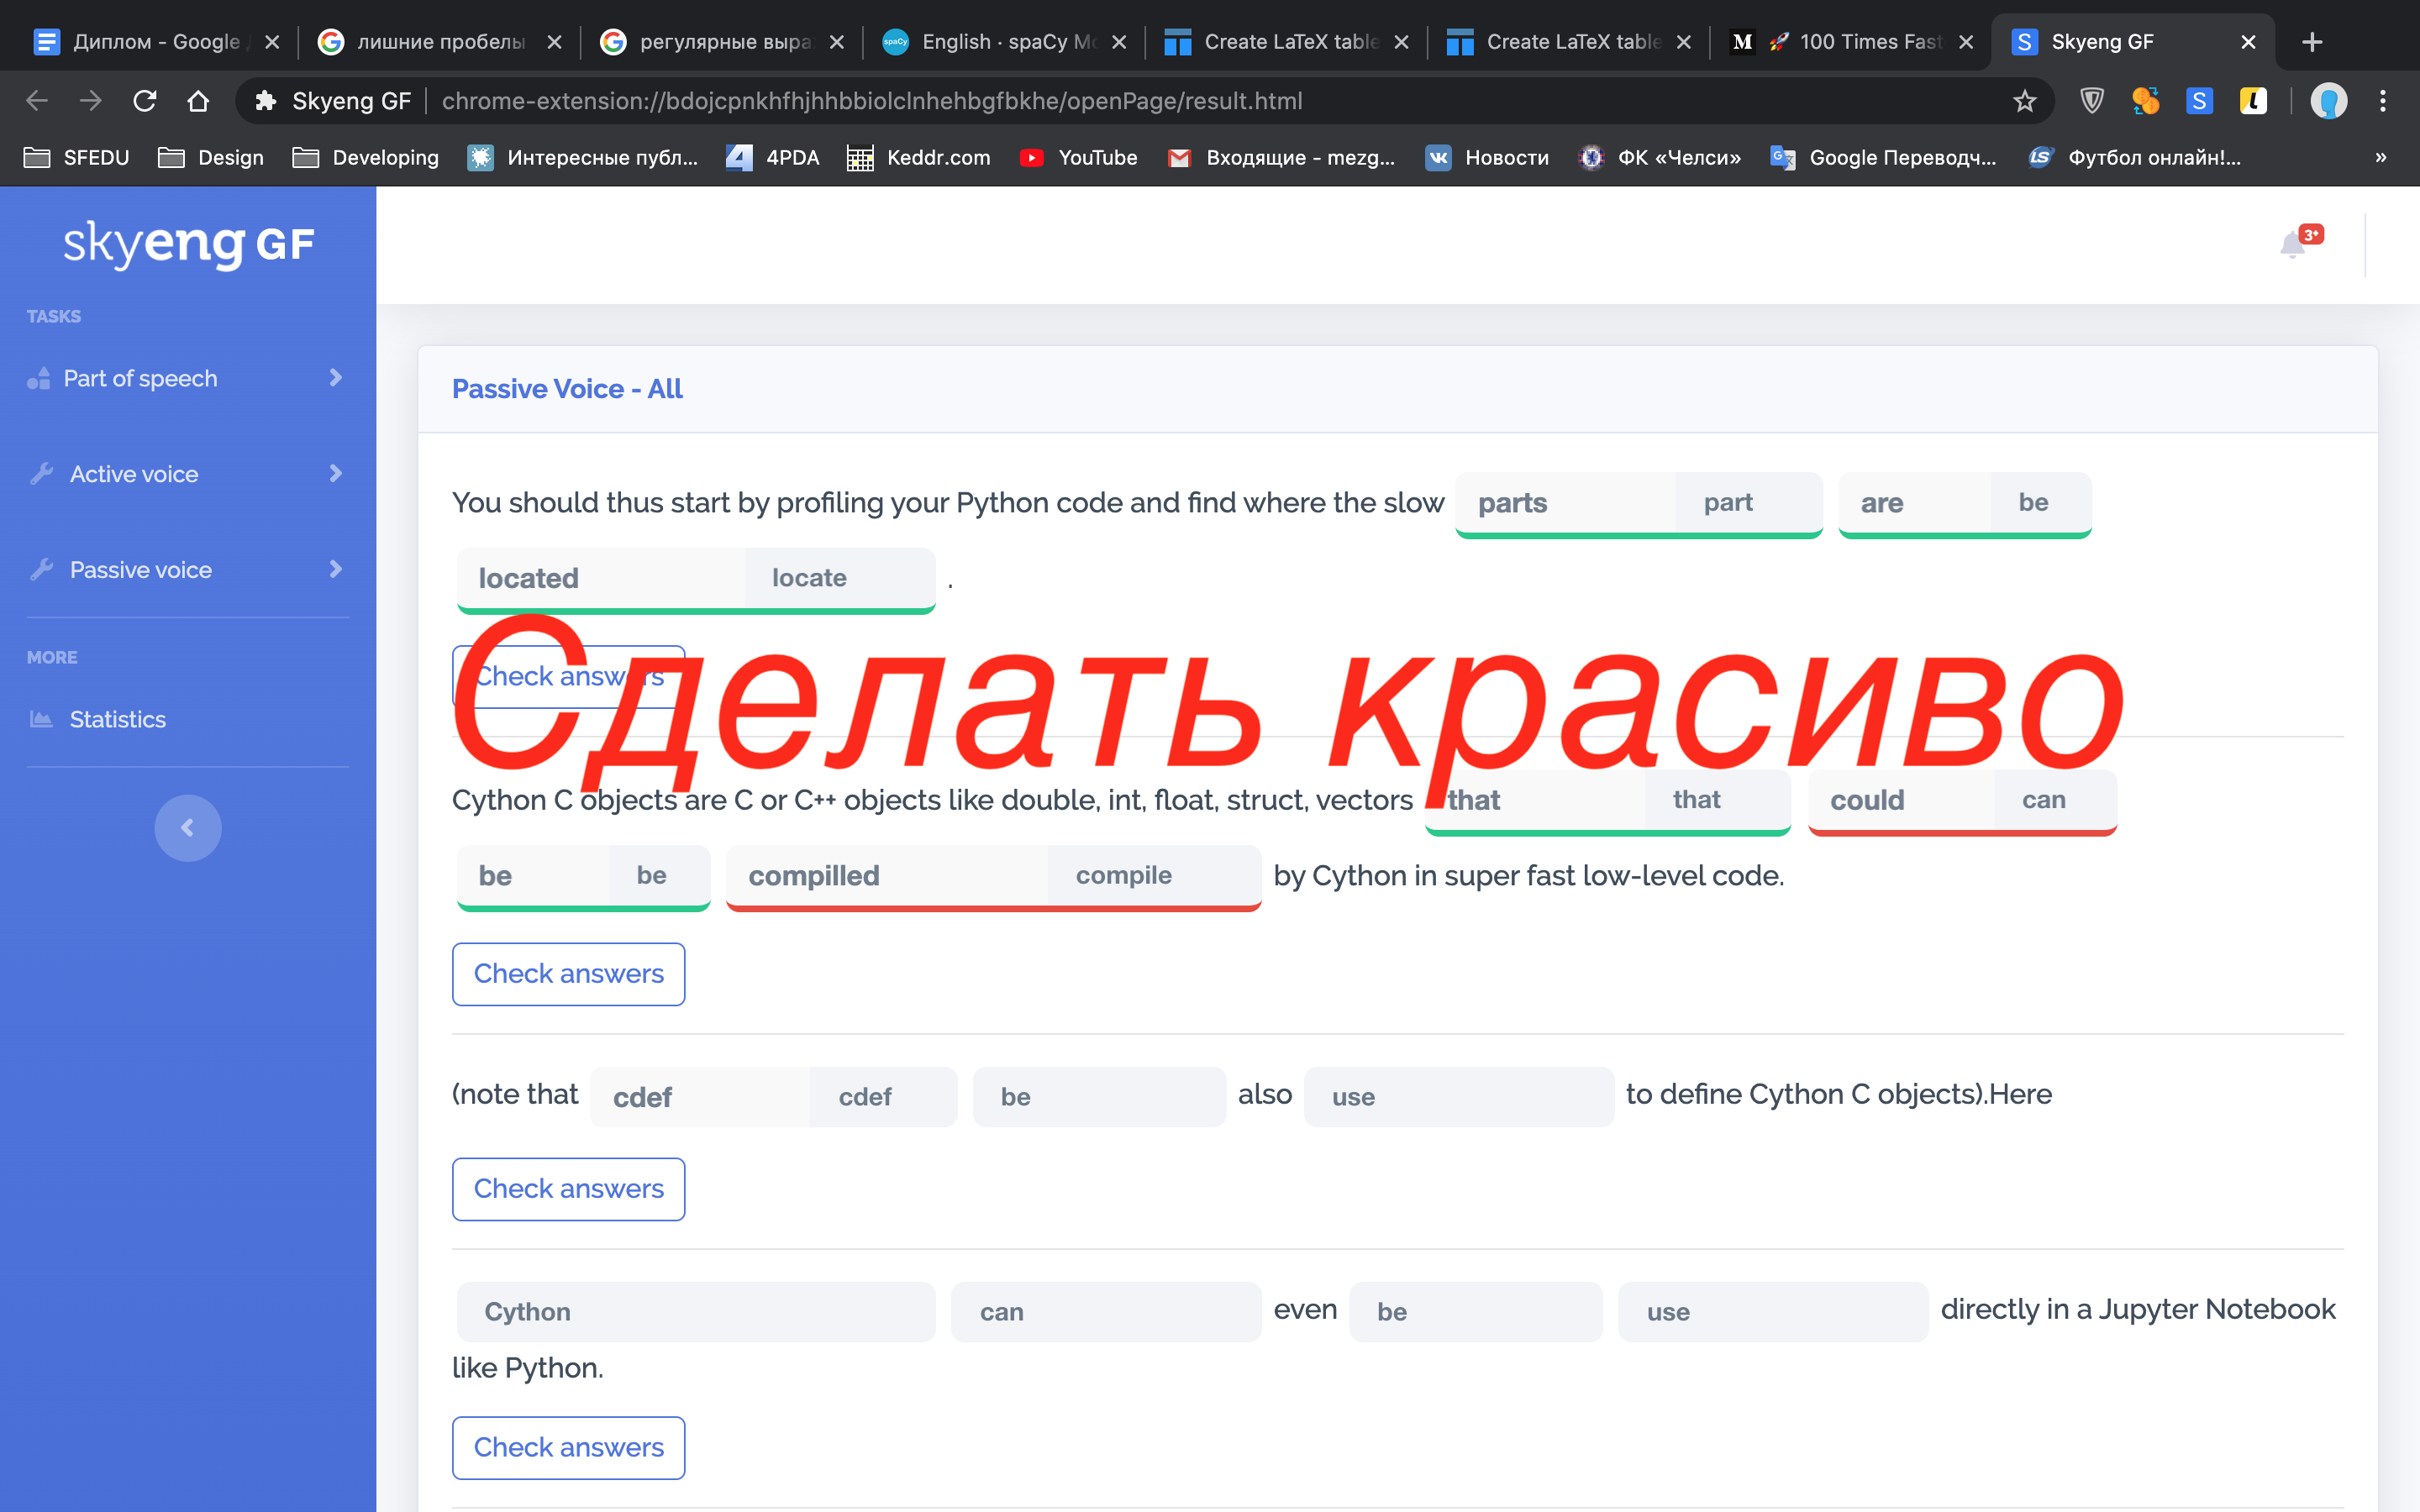
\includegraphics[width=\textwidth]{img/tasks-example}
\caption{\label{fig:tasks-example}Страница со сформированными заданиями}
\end{figure}


%%%%%%%%%%%%%%%%%%%%%%%%%%%%%%%%%%%%%%%
\newpage

\subsection{Используемые инструменты и оборудование}
Для обработки текста и поиска необходимых грамматических конструкций была использована связка модели машинного обучения и Rule-Based алгоритма, который применялся к полученным моделью атрибутам.

В выборе инструментов обработки текстовых данных скорость работы была первоочередным приоритетом ввиду того, что система является клиенто-ориентированной и требует достижения минимального времени на обработку и передачу данных. В Таблице ~\ref{tab:nlp-speed} приведено сравнение времени работы различных библиотек для ряда задач.

Исходя из результатов было принято решение остановиться на \emph{spaCy}. Кроме того, данная библиотека обладает обширной документацией, что облегчает работу с ее компонентами.

\begin{table}
\centering
\caption{\label{tab:nlp-speed}Сравенение выстродействия NLP библиотек}
\begin{tabular}{@{}cccc@{}}
\toprule
SYSTEM  & TOKENIZE & TAG   & PARSE \\ \midrule
spaCy   & 0.2ms    & 1ms   & 19ms  \\
CoreNLP & 0.18ms   & 10ms  & 49ms  \\
ZPar    & 1ms      & 8ms   & 850ms \\
NLTK    & 4ms      & 443ms & n/a   \\ \bottomrule
\end{tabular}
\end{table}

Для развертывания сервера был выбран микрофреймворк \emph{Flask}, который использует набор инструментов Werkzeug и шаблонизатор Jinja2. При этом он обладает достаточной производительностью и совместим с \emph{Python 3.x}, что позволяет использовать его вместе с \emph{spaCy}.

Характеристики сервера следующие:
\begin{itemize}
  \item Memory: ~16GB
  \item Processor: ~Intel Core i5-8400 CPU @ 2.80GHz x6
  \item Graphics: ~GeForce GTX 1070/PCIe/SSE2
  \item OS: Ubuntu 18.04.4 LTS
\end{itemize}
%%%%%%%%%%%%%%%%%%%%%%%%%%%%%%%%%%%%%%%%
\newpage
\subsection{Получение текстовых данных}
Текстовые данные получаются путем их извлечения из html-файла. Для этого производятся следующие операции:
\begin{itemize}
  \item удаление информации за пределами тега $<$body$>$ (см.~листинг~\ref{list:getStrippedBody});
  \item очистка от тегов;
  \item очистка от скриптов
  \item очистка от номеров с общими суффиксами;
  \item очистка от изображений.
\end{itemize}

 Для работы с подстроками используются правила, основанные на регулярных выражениях.

\begin{ListingEnv}[h]
\begin{lstlisting}

getStrippedBody: function (html) {
  let body = html.match(/<body[^>]*>(?:([^]*)<\/body>([^]*)|([^]*))/i);
  if (body && body.length > 1) {
  if (body[2] && body[2].length > this.minBodyTailLength()) {
        body = body[1] + ' ' + body[2];
      } else if (body[1] === undefined) {
                body = body[3];
            } else {
                body = body[1];
            }
        } else {
            body = html;
        }

        return body.replace(/<script\b[^>]*(?:>[^]*?<\/script>|\/>)/ig, '<blink/>');
    },
\end{lstlisting}
\caption{Удаление информации за пределами тега $<$body$>$}
% далее метка для ссылки:
\label{list:getStrippedBody}
\end{ListingEnv}



%%%%%%%%%%%%%%%%%%%%%%%%%%%%%%%%%%%%%%%%
\newpage
\subsection{Модель машинного обучения}
Для извлечения атрибутов, которые необходимы для применения Rule-Based алгоритма, было принято решение использовать сверточную нейронную сеть, принципы работы которой были разобраны в пункте 2.1.

В ходе выбора архитектуры были проанализированы предобученные многозадачные нейронные сети \emph{en\_core\_web\_sm} и  \emph{en\_core\_web\_lg}, обученные на OntoNotes 5. После их применения элементам текста присваиваются метки, обозначающие части речи (TAGGER), синтаксические отношения между словами (PARSER) и именованные сущности (NER).

Основное отличие состоит в применении метода GloVe \autocite{pennington2014glove} для векторного представления слов в \emph{en\_core\_web\_lg}. Данный метод комбинирует в себе принципы word2vec (см. пункт 1.2.3) и SVD-разложения. В то же время архитектура \emph{en\_core\_web\_sm} использует Bloom Embeddings \autocite{DBLP:journals/corr/SerraK17}, что позволяет существенно сократить вес модели, однако влечет за собой значительное снижение сохранения семантических связей. 

Сравнение основных показателей до применения методов Transfer Learning можно видеть в таблице ~\ref{tab:nlp-characteristics}.

\begin{table}
\centering
\caption{\label{tab:nlp-characteristics}Сравнение скорости работы NLP библиотек}
\begin{tabular}{@{}lcccccc@{}}
\toprule
MODEL             & VERSION & LAS   & UAS   & NER F & POS   & SIZE  \\ \midrule
en\_core\_web\_sm & 2.2.5   & 89.71 & 91.62 & 85.55 & 97.05 & 35MB  \\
en\_core\_web\_lg & 2.2.5   & 90.17 & 92.01 & 86.55 & 97.22 & 812MB \\ \bottomrule
\end{tabular}
\end{table}
Основную роль для задачи поиска грамматических конструкций играет правильное построение дерева зависимостей, поэтому главным показателем в приведенной таблице является LAS (анг. Labeled Attachment Score).

Также были проведены тесты для измерения скорости их работы. Для теста были взяты тексты средней длины (порядка 20 000 символов) и проведены замеры скорости работы на 50 итерациях. После этого результаты были округлены. Результаты представлены на таблице ~\ref{tab:models-speed}.

\begin{table}
\centering
\caption{\label{tab:models-speed}Сравнение скорости работы моделей}
\begin{tabular}{@{}lcccc@{}}
\toprule
MODEL             & Loading & Preparation & Text Processing & Full Time \\ \midrule
en\_core\_web\_sm & 0.59028 & 2.4e-5      & 0.51975         & 1.11307   \\
en\_core\_web\_lg & 8.51049 & 2.3e-5      & 0.47446         & 8.98792   \\ \bottomrule
\end{tabular}
\end{table}

Как мы видим, наиболее затратным по времени является этап загрузки модели, а не момент ее применения. Таким образом, в случае предварительной загрузки на сервере, выбор большей модели не скажется на времени отклика работы программы.

При этом применение модели \emph{en\_core\_web\_lg} показывает рост точности определения семантических и синтаксических связей между членами предложения, что позволяет более точно находить грамматические конструкции в предложениях со сложной структурой. 

Следовательно, окончательным выбором стала модель \emph{en\_core\_web\_lg}.


%%%%%%%%%%%%%%%%%%%%%%%%%%%%%%%%%%%%%%%
\subsection{Предварительная обработка текста и настройка модели}
Базовая очистка текста включает в себя удаление нестандартных символов, в том числе различных дефисов (см. листинг \ref{list:clean-text}), смайлов, излишних пробелов. Удаление стоп-слов (предлоги, суффиксы, причастия и пр.) не производится ввиду необходимости сохранения начальной структуры предложения для последующего формирования упражнений.

\begin{ListingEnv}[h]
\begin{lstlisting}
def replace_canadian_period(text):
    text = text.replace(u"\u1427", ".")
    return text


def replace_fancy_hyphens(text):
    hlist = [u"\u002d", u"\u058a", u"\u058b", u"\u2010",
             u"\u2011", u"\u2012", u"\u2013", u"\u2014", 
             u"\u2015", u"\u2e3a", u"\u2e3b", u"\ufe58", 
             u"\ufe63", u"\uff0d"]
    for h in hlist:
        text = text.replace(h, "-")
    return text


def lexical_processor(text):
    text = os.linesep.join([s for s in text.splitlines() if s])
    text = replace_canadian_period(text)
    text = replace_fancy_hyphens(text)
    return text
\end{lstlisting}
\caption{Предварительная очистка текста}
% далее метка для ссылки:
\label{list:clean-text}
\end{ListingEnv}

Этап настройки модели состоит в применение нестандартных правил для компонентов \emph{Tokenizer} и \emph{Matcher}. Данные меры необходимы для корректного отображения токенов при формировании заданий. 

В случае \emph{Tokenizer} был изъят дефис из набора символов, которые разделяют слово на части: например, слово “semi-controlled” при изначальных настройках делится на токены ''semi'', ''-'', ''controlled”.


Для компонента \emph{Matcher} были добавлены правила, которые позволяют собрать токены, обозначающие сокращенное написание слов ''am'', ''have'' в один: например, конструкции ''I’m'' и ''I've'' при изначальных настройках делится на токены ''I'', '' ' '', ''m'' и ''I'', '' ' '', ''ve'' соответственно. 


\begin{ListingEnv}[h]
\begin{lstlisting}
    # Change tokenizer of the NLP Model.
    infixes = (
            LIST_ELLIPSES
            + LIST_ICONS
            + [
                r"(?<=[0-9])[+\-\*^](?=[0-9-])",
                r"(?<=[{al}{q}])\.(?=[{au}{q}])".format(
                    al=ALPHA_LOWER, au=ALPHA_UPPER,
                    q=CONCAT_QUOTES
                ),
                r"(?<=[{a}]),(?=[{a}])".format(a=ALPHA),
                r"(?<=[{a}0-9])[:<>=/](?=[{a}])".format(a=ALPHA),
            ]
    )
    infix_re = compile_infix_regex(infixes)

    # Change matcher of the NLP Model
    matcher = Matcher(nlp.vocab)
    pattern = [{'ORTH': "'"},
               {'ORTH': 've'}]
    pattern_2 = [{'ORTH': "'"},
                 {'ORTH': 'm'}]

    matcher.add('QUOTED', None, pattern, pattern_2)
\end{lstlisting}
\caption{Модификация компонентов \emph{Tokenizer} и  \emph{Matcher}}
% далее метка для ссылки:
\label{list:tokenizer-matcher}
\end{ListingEnv}

После применения дополнительных правил разбиения и форматирования (см.~листинг.~\ref{list:tokenizer-matcher}) текст становится приемлемым для визуализации пользователю.

%%%%%%%%%%%%%%%%%%%%%%%%%%%%%%%%%%%%%%%
\subsection{Построение алгоритма поиска грамматических конструкций}
Для поиска грамматических конструкций используется алгоритм, основанный на навигации по дереву зависимостей. Оно может быть построено на основе наборов признаков, которые формируются для каждого члена предложения в ходе применения модели. К таким признакам относятся: 
\begin{itemize}
  \item Text: оригинальный текст слова.
  \item Lemma: начальная форма слова.
  \item POS: простая метка части речи по модели UPOS.
  \item Tag: подробная метка части речи.
  \item Dep: синтаксическая зависимость, связь между токенами.
  \item Shape: форма слова - заглавные буквы, знаки препинания, цифры.
  \item Is alpha: состоит ли токен из буквенных символов?
  \item Is stop: является ли токен частью стоп-листа, то есть наиболее распространенных слов языка?
\end{itemize}

Рассмотрим пример построения признаков для следующего предложения:
“Apple is looking at buying U.K. startup”. Таблица~\ref{tab:spacy-example-attr} демонстрирует результат применения модели \emph{en\_core\_web\_lg}.

На базе полученных данных может быть построено дерево зависимостей, пример приведен на рисунке ~\ref{fig:sentence}.

\begin{figure}[h]
\centering
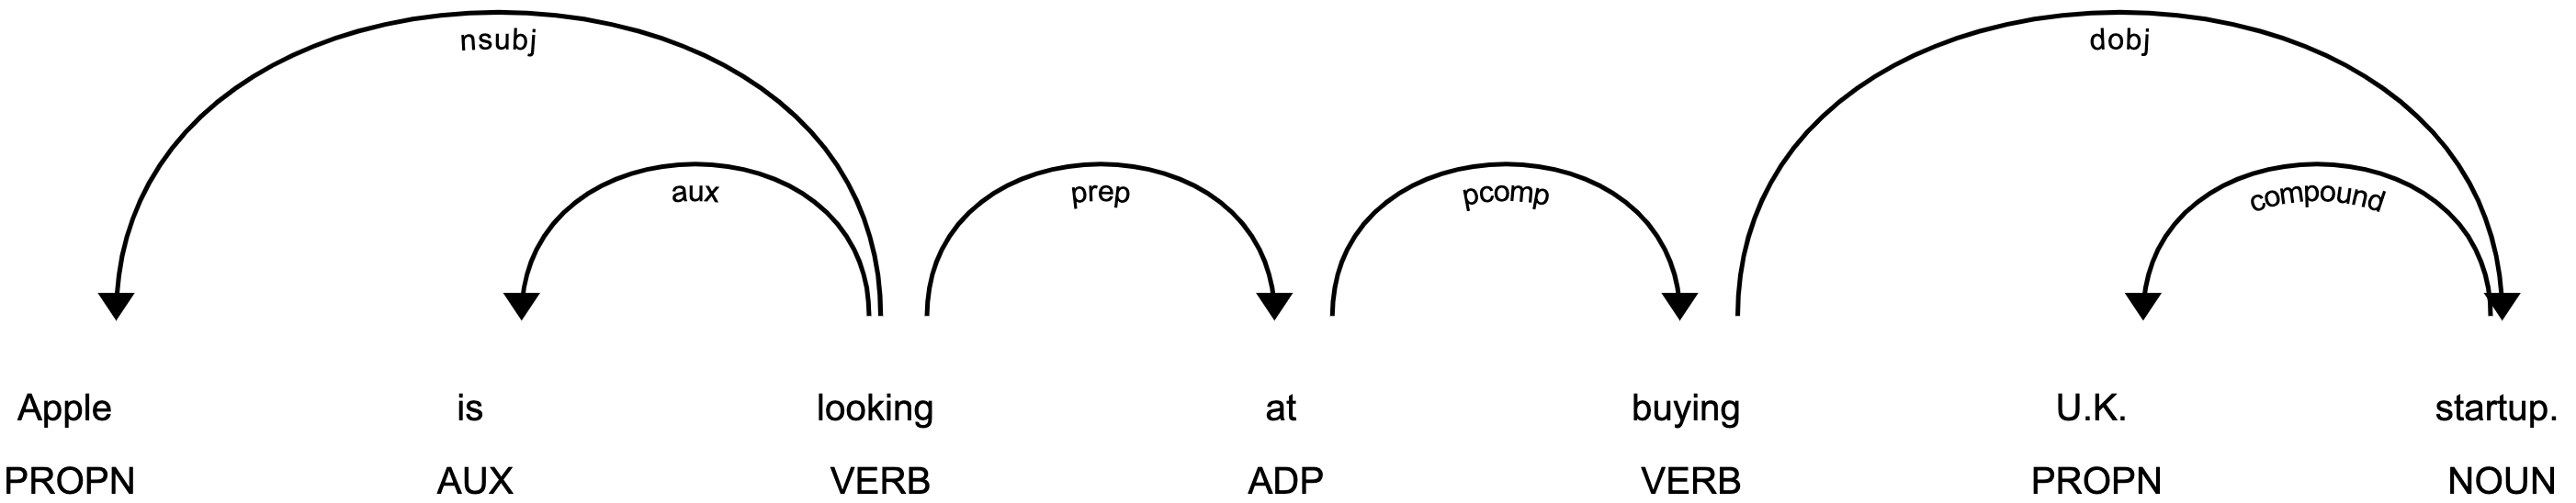
\includegraphics[width=\textwidth]{img/sentence}
\caption{\label{fig:sentence}Пример построения дерева зависимостей}
\end{figure}

\begin{table}
\centering
\caption{\label{tab:spacy-example-attr}Признаки, полученные моделью \emph{en\_core\_web\_lg}}
\begin{tabular}{@{}cccccccc@{}}
\toprule
TEXT    & LEMMA   & POS   & TAG & DEP      & SHAPE & ALPHA & STOP  \\ \midrule
Apple   & apple   & PROPN & NNP & nsubj    & Xxxxx & True  & False \\
is      & be      & VERB  & VBZ & aux      & xx    & True  & True  \\
looking & look    & VERB  & VBG & ROOT     & xxxx  & True  & False \\
at      & at      & ADP   & IN  & prep     & xx    & True  & True  \\
buying  & buy     & VERB  & VBG & pcomp    & xxxx  & True  & False \\
U.K.    & u.k.    & PROPN & NNP & compound & X.X.  & False & False \\
startup & startup & NOUN  & NN  & dobj     & xxxx  & True  & False \\ \bottomrule
\end{tabular}
\end{table}

Далее были построены наборы правил, которые задают необходимые шаблоны, ориентированные на распознание различных грамматических конструкций. Для детекции \emph{Active} и \emph{Passive Voice} основными атрибутами при построении правил стали соответствия \emph{auxiliary verb (aux)}, \emph{passive auxiliary of a clause (auxpass)}, \emph{verb tag}, а также соответствие набору зависимостей.

Паттерны были сформированы на основе формальной грамматики английского языка с учетом особенностей применяемых статистических моделей. Пример таких правил представлен в таблице ~\ref{tab:passive}.

\begin{table}
\centering
\caption{\label{tab:passive}Шаблоны для детекции конструкций \emph{Passive Voice}}
\begin{tabular}{@{}cccc@{}}
\toprule
TASK                       & AUX                                                                 & AUXPASS                                                & NUMBER OF AUX \\ \midrule
Present Simple             & n/a                                                                 & \begin{tabular}[c]{@{}c@{}}am, is,\\  are\end{tabular} & 0             \\
Present Continuous         & \begin{tabular}[c]{@{}c@{}}am, is, \\ are\end{tabular}              & being                                                  & 1             \\
Present Perfect            & \begin{tabular}[c]{@{}c@{}}have, \\ has\end{tabular}                & been                                                   & 1             \\
Future In The Past Perfect & \begin{tabular}[c]{@{}c@{}}should, would, \\ have, has\end{tabular} & been                                                   & 2             \\ \bottomrule
\end{tabular}
\end{table}

Следующий этап -- навигация по дереву зависимостей. Результатом работы алгоритма должны стать массивы найденных фраз, их индексов, восстановленных начальных форм, POS тегов и тегов зависимостей слов, входящих в найденные фразы, а также предложений, к которым они относятся. 

Обобщенный алгоритм поиска состоит из следующих этапов:

\begin{enumerate}
  \item Создание массивов, которые соответствуют ожидаемым результатам.
  \item Навигация по предложениям в тексте.
  \item Поиск корневого слова в предложении.
  \item Создание локальных массивов, относящихся к данному предложению.
  \item Навигация по словам, зависящим от корневого.
  \item Проверка соответствия зависимых слов набору правил.
  \item Добавление подходящих слов в локальные массивы.
  \item Контрольная проверка найденных соответствий общему шаблону.
  \item Переход к действиям в зависимости от результата:
  \begin{enumerate}[label*=\arabic*.]
      \item При соответствии общему шаблону добавить найденную информацию в общие массивы.
      \item При несоответствии общему шаблону обнулить массивы и прервать навигацию по зависимым словам.
    \end{enumerate}
 \item Продолжение навигации по следующим предложениям.
\end{enumerate}

Момент обработки \emph{auxiliary verb (aux)} для задания \emph{Passive Voice} приведен на листинге \ref{list:aux}.

\begin{ListingEnv}[h]
\begin{lstlisting}
# 3: An auxiliary of a clause
if child.dep_ == 'aux':
    if child_lower in tense_rule.get('aux'):
        num_of_aux += 1
        passive_match.append(child.text)
        passive_match_lexemes.append(child.lemma_)
        passive_match_indices.append([
                child.idx - sent.start_char,
                child.idx + len(child) - sent.start_char])
        passive_match_pos.append(child.pos_)
        passive_match_dep.append(child.dep_)

        # Exception handling with Modals
        if tense == 'MODALS' and child_lower == 'have':
            num_of_aux_rule += 1
    else:
     # If we find a match but from another tense => skip
     passive_match = []
     passive_match_lexemes = []
     passive_match_indices = []
     passive_match_pos = []
     passive_match_dep = []
     num_of_aux = 0
     num_of_aux_rule = tense_rule.get('num_of_aux')
     break
\end{lstlisting}
\caption{Обработка \emph{'aux'} при поиске конструкций \emph{Passive Voice}}
% далее метка для ссылки:
\label{list:aux}
\end{ListingEnv}

Полученные данные отправляются на сторону клиента для дальнейшей обработки и формирования упражнений.
%%%%%%%%%%%%%%%%%%%%%%%%%%%%%%%%%%%%%%%
\newpage
\subsection{Формирование упражнений}
Кратко рассмотрим механизм формирования и визуализации упражнений.

Полученная информация с найденными фразами, лексемами, индексами и их предложениями передается в функцию, которая создает блоки с упражнениями. Каждый такой блок представляет собой <div> элемент, который хранит информацию о типе задания, порядковом номере упражнения, а также содержит поля ввода, которые вставляются на места слов, входящих в состав найденных фраз. Для помощи пользователю вставляются восстановленные начальные формы вырезанных слов.

Работа над формированием блоков ведется путем редактирования строк, которые представляют собой блоки html кода. После окончательного формирования элемента производится его интеграция на открытую страницу. Для такой работы с html используется класс htmlString, который входит в состав Jquery.

Пример сформированного блока можно увидеть на листинге \ref{list:html}.

\begin{ListingEnv}[h]
\begin{Verb}
<div class="task-p">
<p>You should thus start by profiling your Python code and find
 where the slow
    <label class="input__label" for="task-0-0">
        <span class="input__label-content">part</span>
    </label>
    
    <label class="input__label" for="task-0-1">
        <span class="input__label-content ">be</span>
    </label>

    <label class="input__label " for="task-0-2">
        <span class="input__label-content">locate</span>
    </label>
.</p> 
</div>
\end{Verb}
\caption{Пример упрощенной структуры элемента с заданием}
% далее метка для ссылки:
\label{list:html}
\end{ListingEnv}
%%%%%%%%%%%%%%%%%%%%%%%%%%%%%%%%%%%%%%%
\subsection{Сохранение статистики пользователя}
Все вводимые пользователем данные при прохождении упражнений учитываются в статистике. Для ее хранения используется структура Json.  

В ней сохраняется информация о источнике данных (url-адрес), информация о проделанных заданиях, информация о количестве правильных и неправильных ответов для каждого слова с учетом их частей речи и принадлежности к той или иной части предложения. Такие сведения позже могут комбинироваться для предоставления статистики пользователю (см.~рис.~\ref{fig:stats-passive}), а также использоваться для построения рекомендательной системы.

\begin{figure}[ht]
\centering
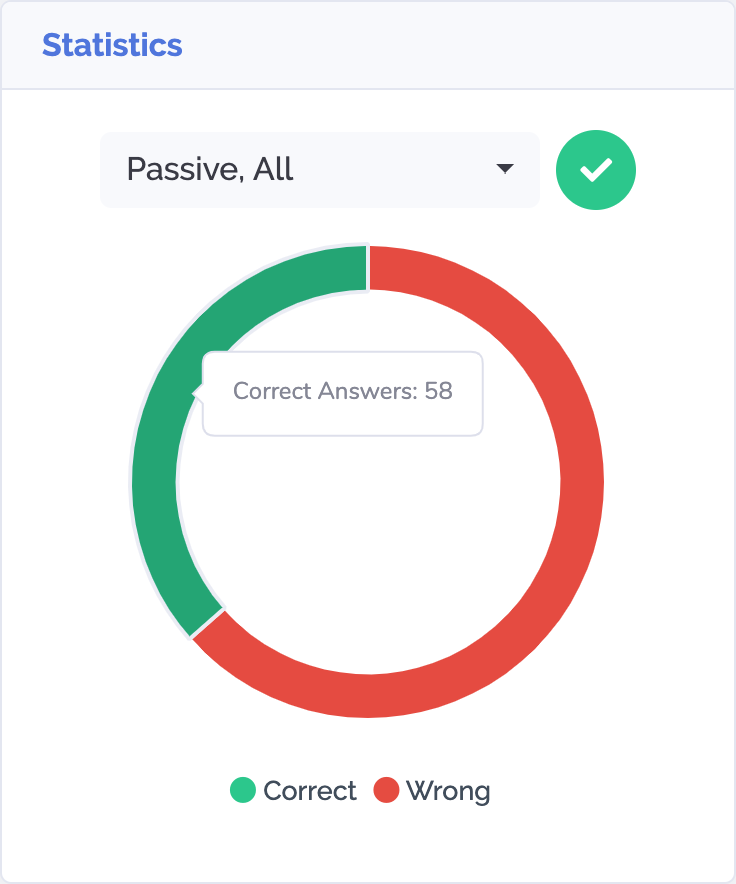
\includegraphics[width=0.4\textwidth]{img/stats}
\caption{\label{fig:stats-passive}Пример визуализации статистики}
\end{figure}

Хранение статистики происходит в веб-браузере путем использования \emph{Window.localStorage}. Данные также дублируются в \emph{NoSQL} базе данных \emph{mongoDB}. Ввиду отсутствия на данный момент этапа авторизации в системе, в качестве идентификатора пользователя используется уникальный идентификатор расширения.

Восстановление данных статистики производится при каждом новом открытии страницы с заданиями. Краткий алгоритм состоит из перечисленных этапов, при этом переход к следующему происходит при неудаче на предыдущем:
\begin{enumerate}
  \item Попытка восстановить данные из \emph{localStorage}.
  \item Попытка восстановить данные из \emph{mongoDB}.
  \item Инициализация новой структуры и запись ее в \emph{localStorage} и \emph{mongoDB}.
\end{enumerate}

Обновление данных внутри \emph{localStorage} происходит после каждого нового ответа пользователя, а запись в удаленную базу данных каждые 5 ответов, чтобы снизить нагрузку на нее и предотвратить задержки в работе приложения.
%%%%%%%%%%%%%%%%%%%%%%%%%%%%%%%%%%%%%%%
\subsection{Повышение производительности системы}
Было произведено тестирование скорости работы модели \emph{en\_core\_web\_lg}. Целью проведения данных тестов стало выявление оптимальных параметров, которые помогают повысить производительность системы.

Были выявлены следующие корреляции:
\begin{itemize}
  \item Зависимость скорости работы от количества пакетов, на которые разбивается входной текст.
  \item Зависимость скорости работы от размера пакетов, на которые разбивается входной текст.
  \item Зависимость скорости работы от выбранного оборудования.
    \item Зависимость скорости работы от размера входного данных.
\end{itemize}

Для проведения тестов использовались тексты, длина которых составляла от 5 000 до 60 000 символов с шагом в 5 000 символов.

Для получения достаточного количества текстов, их формирование происходило на основе датасета CoNLL-2000. Для этого его текст был приведен в удобный для анализа вид, после чего были сформированы группы по 20 текстов каждой длины (для 60 000 символов - 18 текстов).
Таким образом, тестовая выборка составила 238 различных текстов.

Для подвыборки из 20 текстов были проведены начальные тесты, целью которых было выявление разумных границ тестирования.
Полученные  результаты:
\begin{itemize}
  \item Минимальный размер пакета: 700 символов
  \item Максимальный размер пакета: 5000 символов
  \item Шаг: 100 символов
\end{itemize}

На основе полученных данных был произведен полноценный тест. 

Методика тестирования была следующей:
\begin{enumerate}
  \item Каждый из сформированных текстов подавался на вход процедуре тестирования по 5 раз.
  \item Для каждой итерации выполнялись разбиения входных данных на пакеты длиной 700...5000 символов с шагом = 100 (43 итерации).
  \item Полученные значения записывались в csv файл.
  \item Были найдены средние значения результатов времени обработки каждого текста. 
  \item После получения индивидуальных результатов для всех 238 текстов, результаты группировались по длине текстов, к которым они относились.
  \item Были найдены средние значения для сгруппированных результатов. 
  \item Все результаты были проанализированы на предмет выявления зависимостей

  \item Все результаты, как сгруппированные, так и индивидуальные, были визуализированы.
  \item Аналогичные действия были произведены с использованием GPU. 
\end{enumerate}

В сумме было проведено 102 340 замеров (CPU + GPU).

\begin{figure}[ht]
\centering
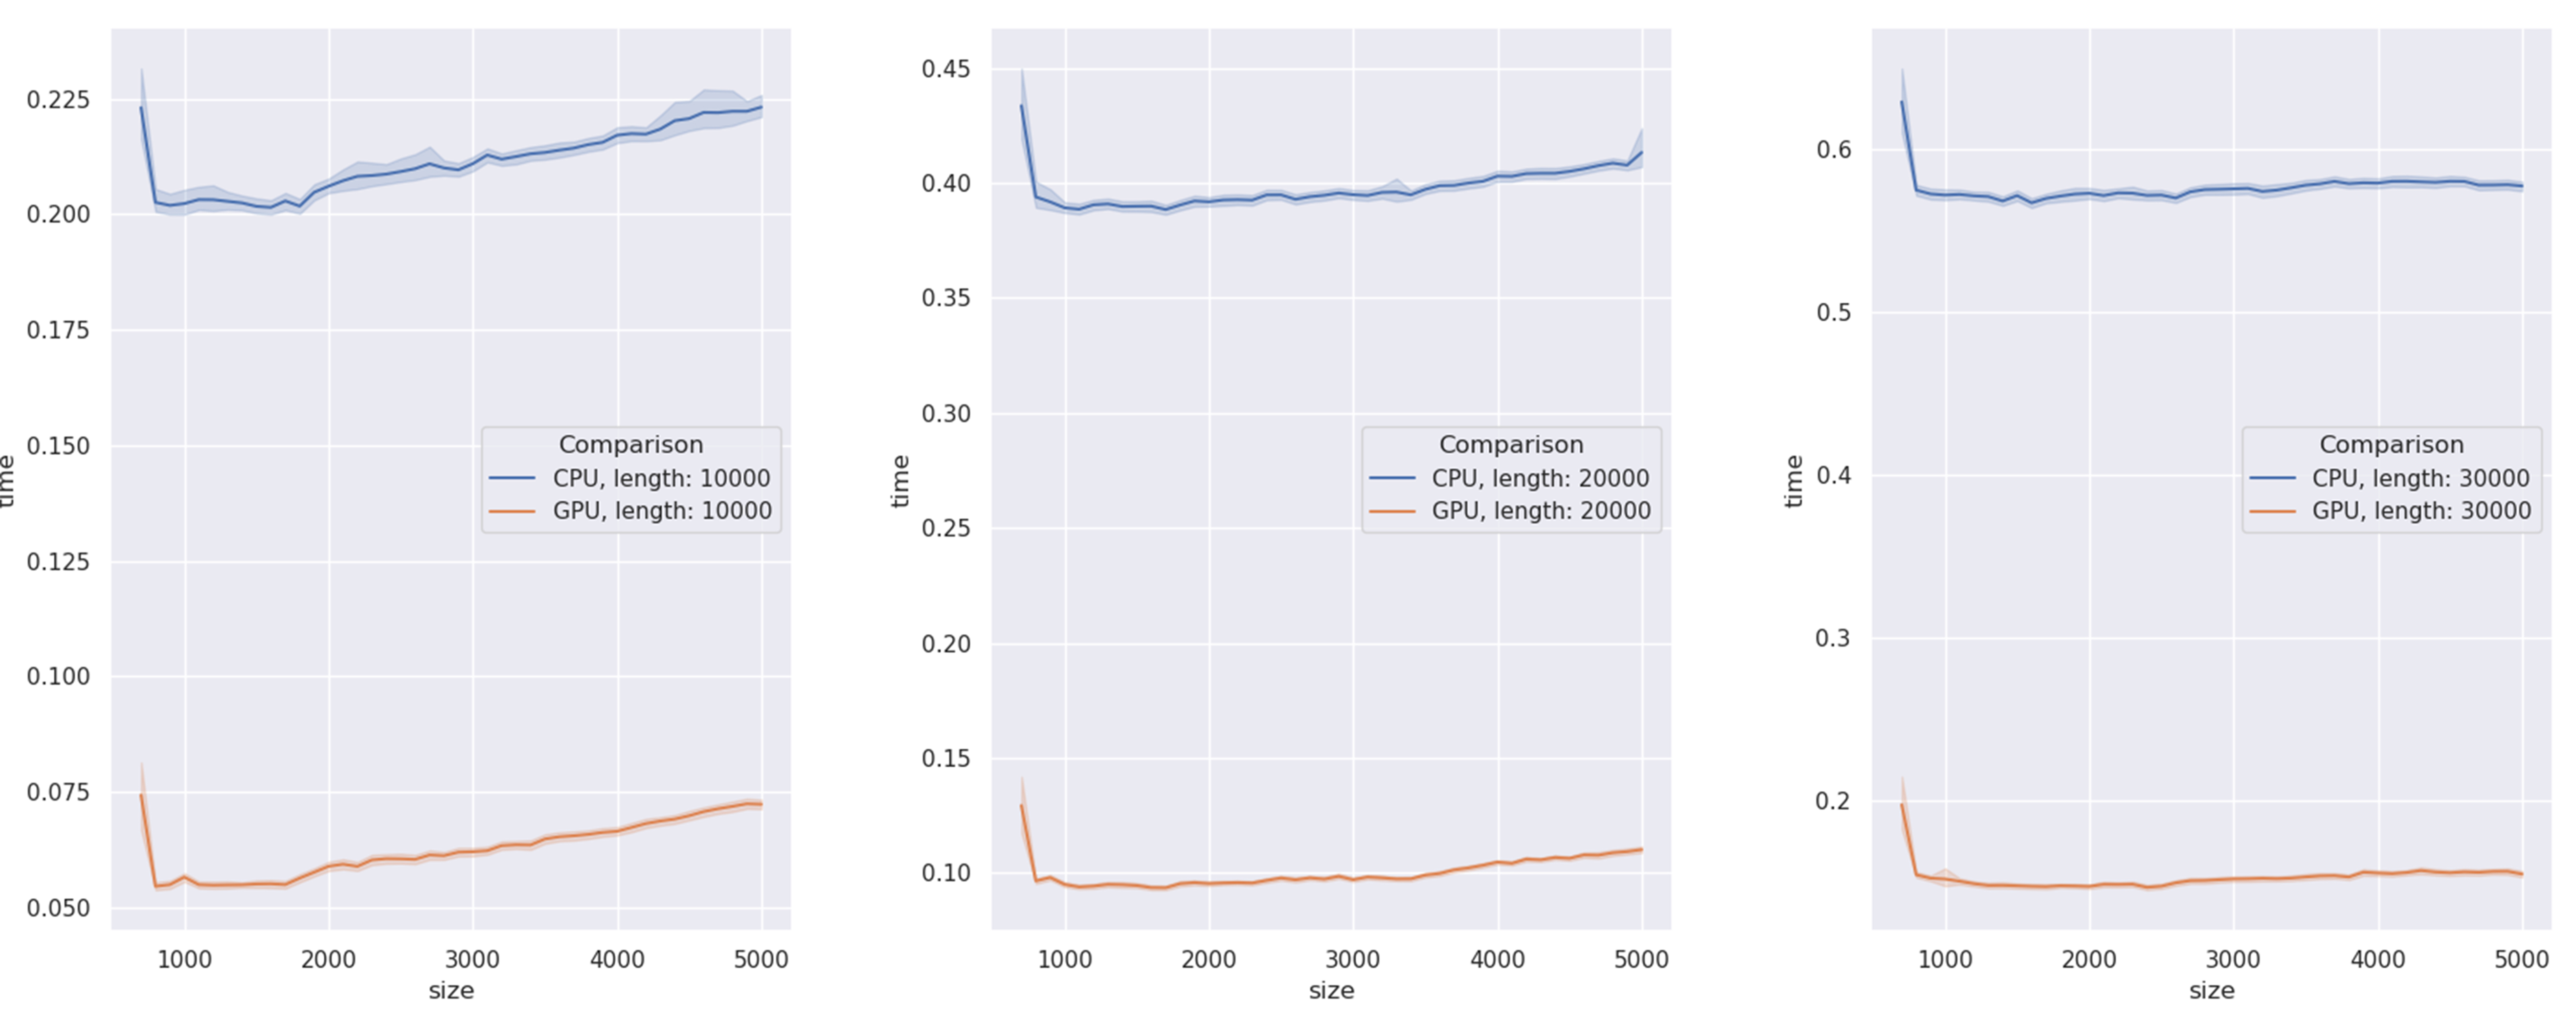
\includegraphics[width=\textwidth]{img/in_text_compare}
\caption{\label{fig:in_text_compare}Результат тестов производительности модели}
\end{figure}

Как мы видим из полученных результатов на рисунке \ref{fig:in_text_compare} (полное сравнение приведено в приложении 1 и приложении 2), основной прирост скорости достигается за счет перехода с CPU на GPU. В отличие от изначального предположения, резкого роста времени работы на диапазоне 1000-5000 символов не наблюдается (отсекаем минимальный размер пакетов, так как из-за их большого количества производительность резко падает), однако проведенные тесты помогают выявить зависимость минимального времени выполнения от размера входных данных (длины текста). 

По результатам теста можно сказать, что для больших текстов (>25K символов), выбор значения в данном промежутке не является принципиальным и следует выбирать больший, так как в дальнейшем алгоритм поиска грамматических конструкций будет работать быстрее за счет меньшего количества итераций цикла (меньше получаемых пакетов). Для малых же текстов правильный выбор параметра из данного промежутка может показать значительный рост производительности в процентном соотношении. 

Полученные данные помогают динамически подбирать параметр разбиения текста на пакеты. Однако при реализации такого подхода требуется учитывать, что граница пакета может попасть на середину слова или предложения. Реализация такого алгоритма представлена в приложении 3.


%%%%%%%%%%%%%%%%%%%%%%%%%%%%%%%%%%%%%%%

\newpage
\Conc

Типа сделал это хуйню:
\begin{itemize}
  \item изучить методы Data Mining и Machine Learning в области обработки естественного языка; 
  \item изучить методы векторного представления слов;
  \item разработать метод предварительной очистки текста;
  \item изучить модели машинного обучения для извлечения необходимых признаков из текста;
  \item разработать алгоритм поиска грамматических конструкций;
  \item разработать алгоритм формирования заданий на основе найденных конструкций;
  \item реализовать развертывание сервера;
  \item разработать web-платформу для взаимодействия с пользователями;
  \item проанализировать возможности повышения производительности системы;
  \item проанализировать возможности повышения точности обнаружения грамматических конструкций;
  \item реализовать базу данных результатов пользователей для ведения статистики.
\end{itemize}
%%%%%%%%%%%%%%%%%%%%%%%%%%%%%%%%%%%%%%%
% Печать списка литературы (библиографии)
\newpage

\printbibliography[%{}
    heading=bibintoc%
    %,title=Библиография % если хочется это слово
]

\newpage
\section*{Оформить как приложение 1}
\label{sec:len}
\addcontentsline{toc}{section}{\nameref{sec:len}}

\begin{figure}[h]
\centering
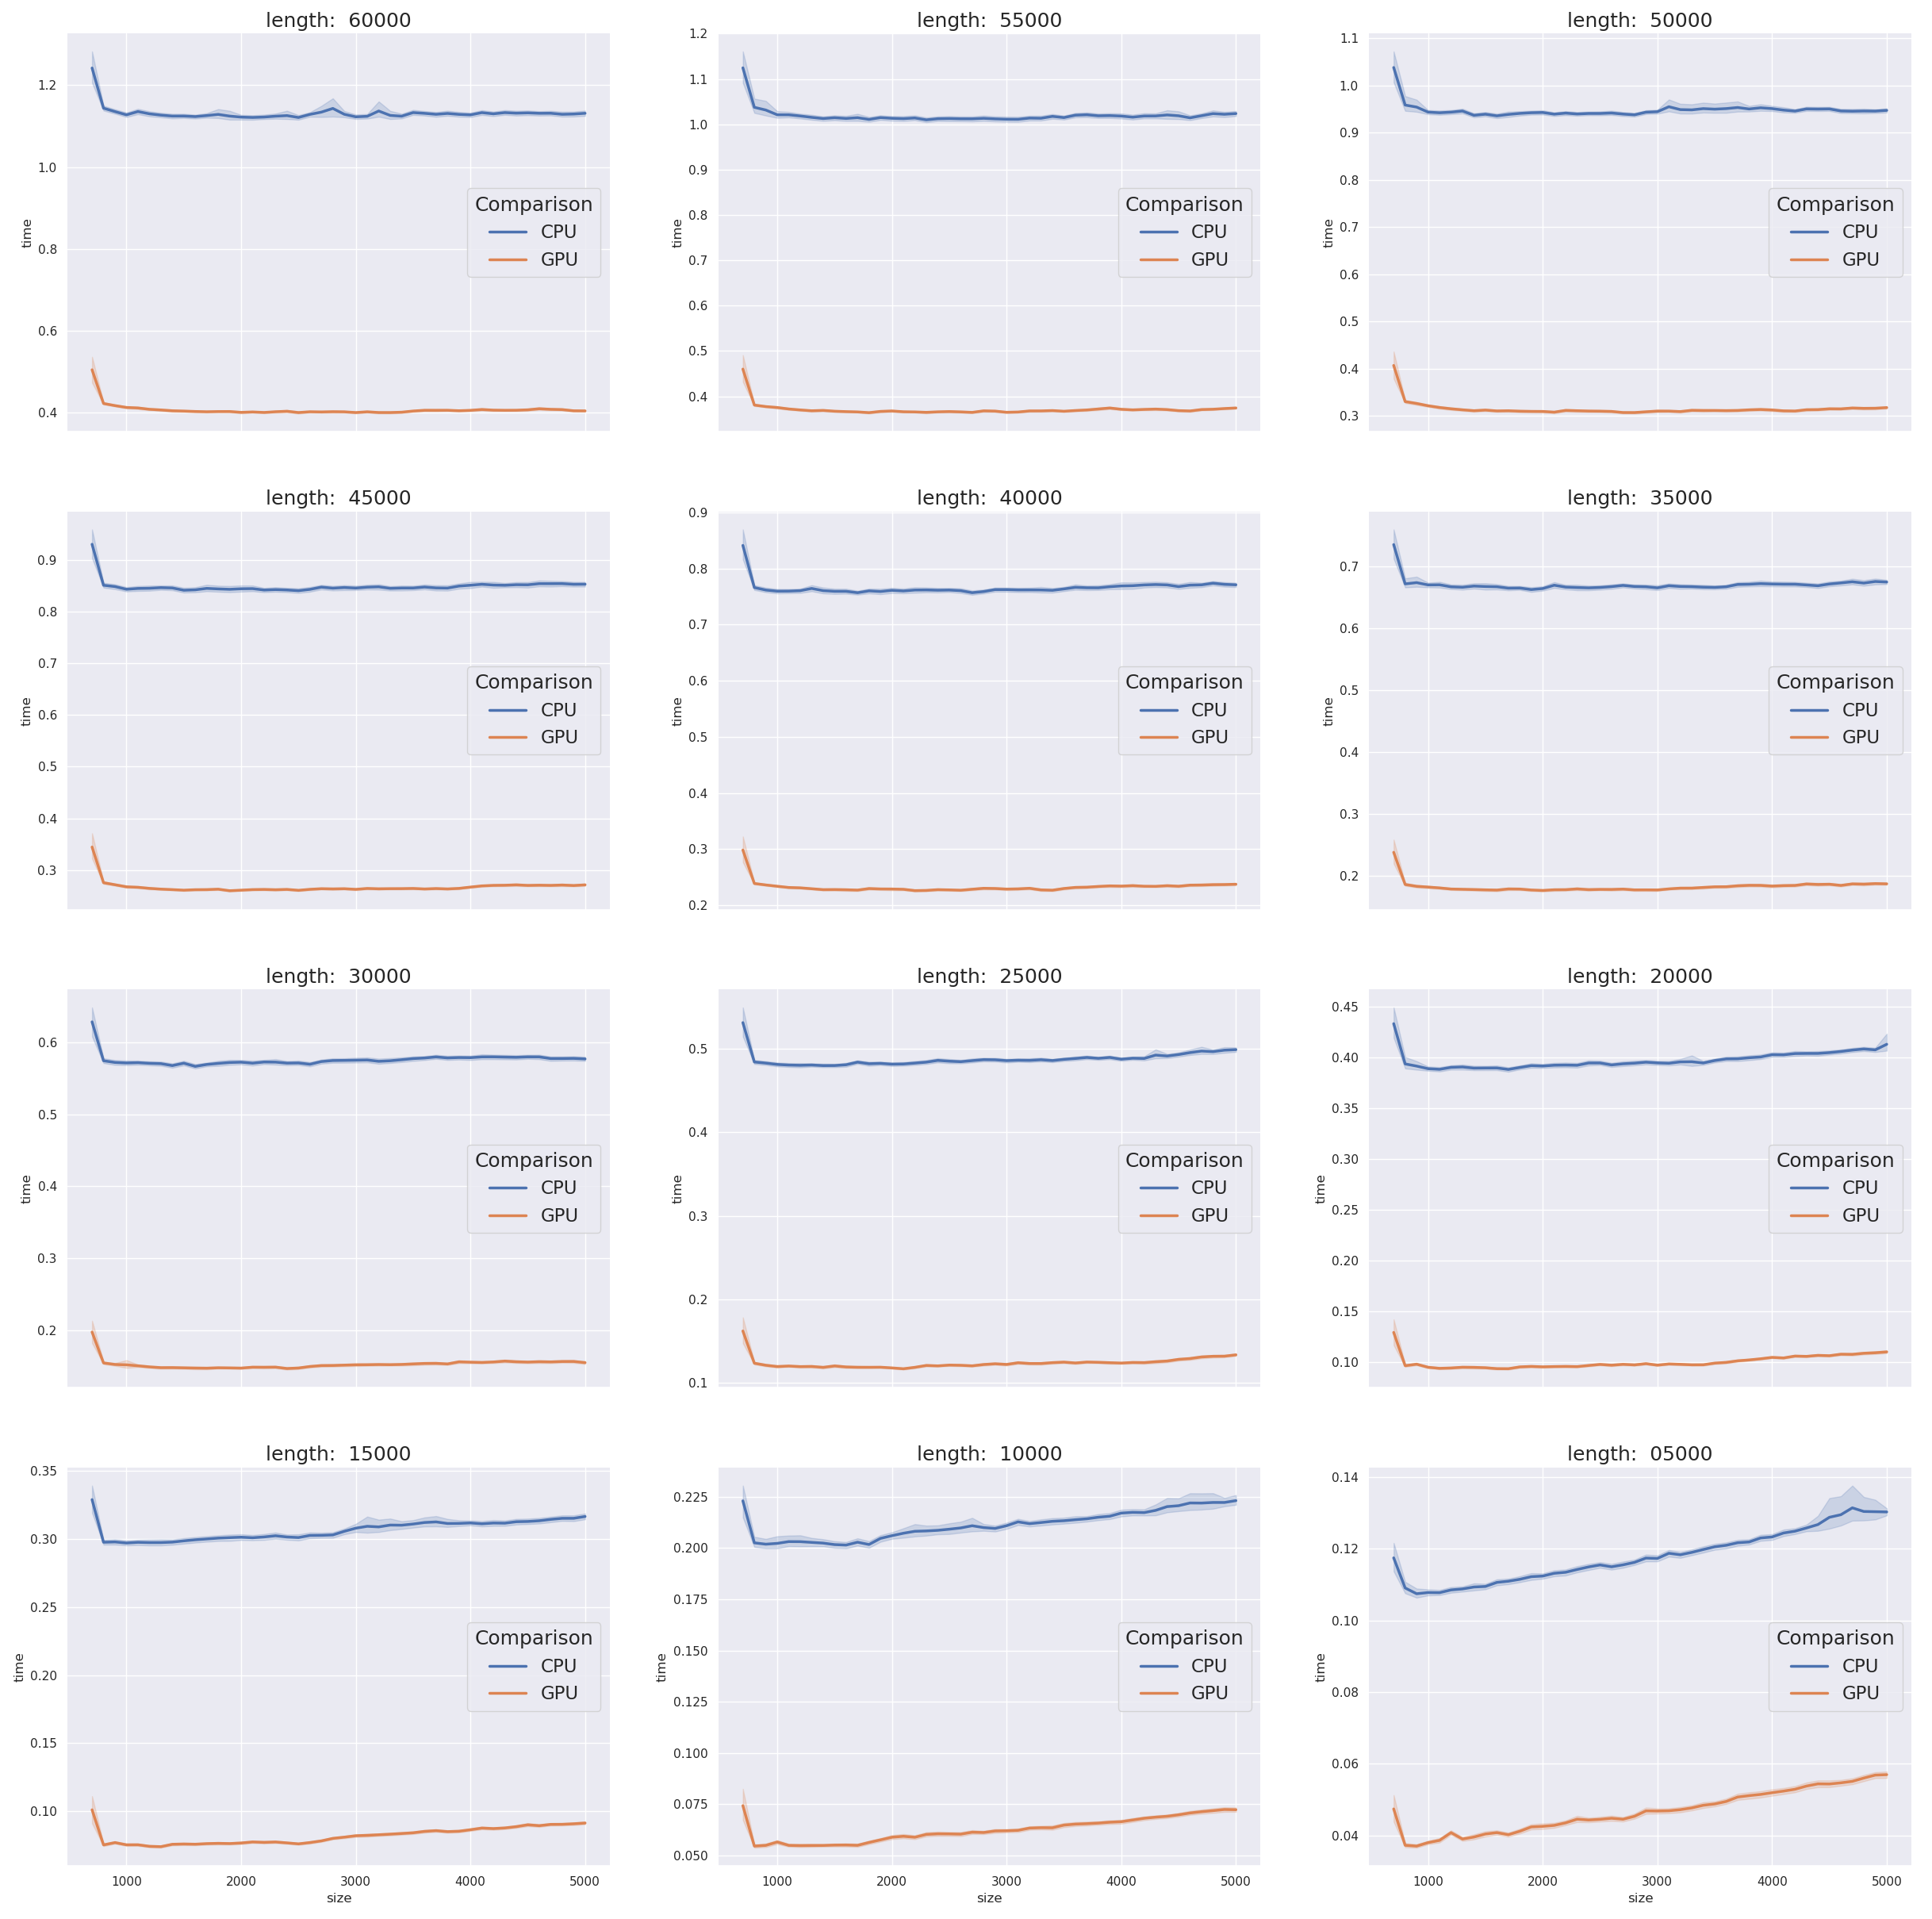
\includegraphics[width=\textwidth]{img/len_CPU_vs_GPU_Grid}
\caption{\label{fig:len_CPU_vs_GPU_Grid}Зависимость времени работы от длины текста}
\end{figure}

\newpage
\section*{Оформить как приложение 2}
\label{sec:num}
\addcontentsline{toc}{section}{\nameref{sec:num}}

\begin{figure}[h]
\centering
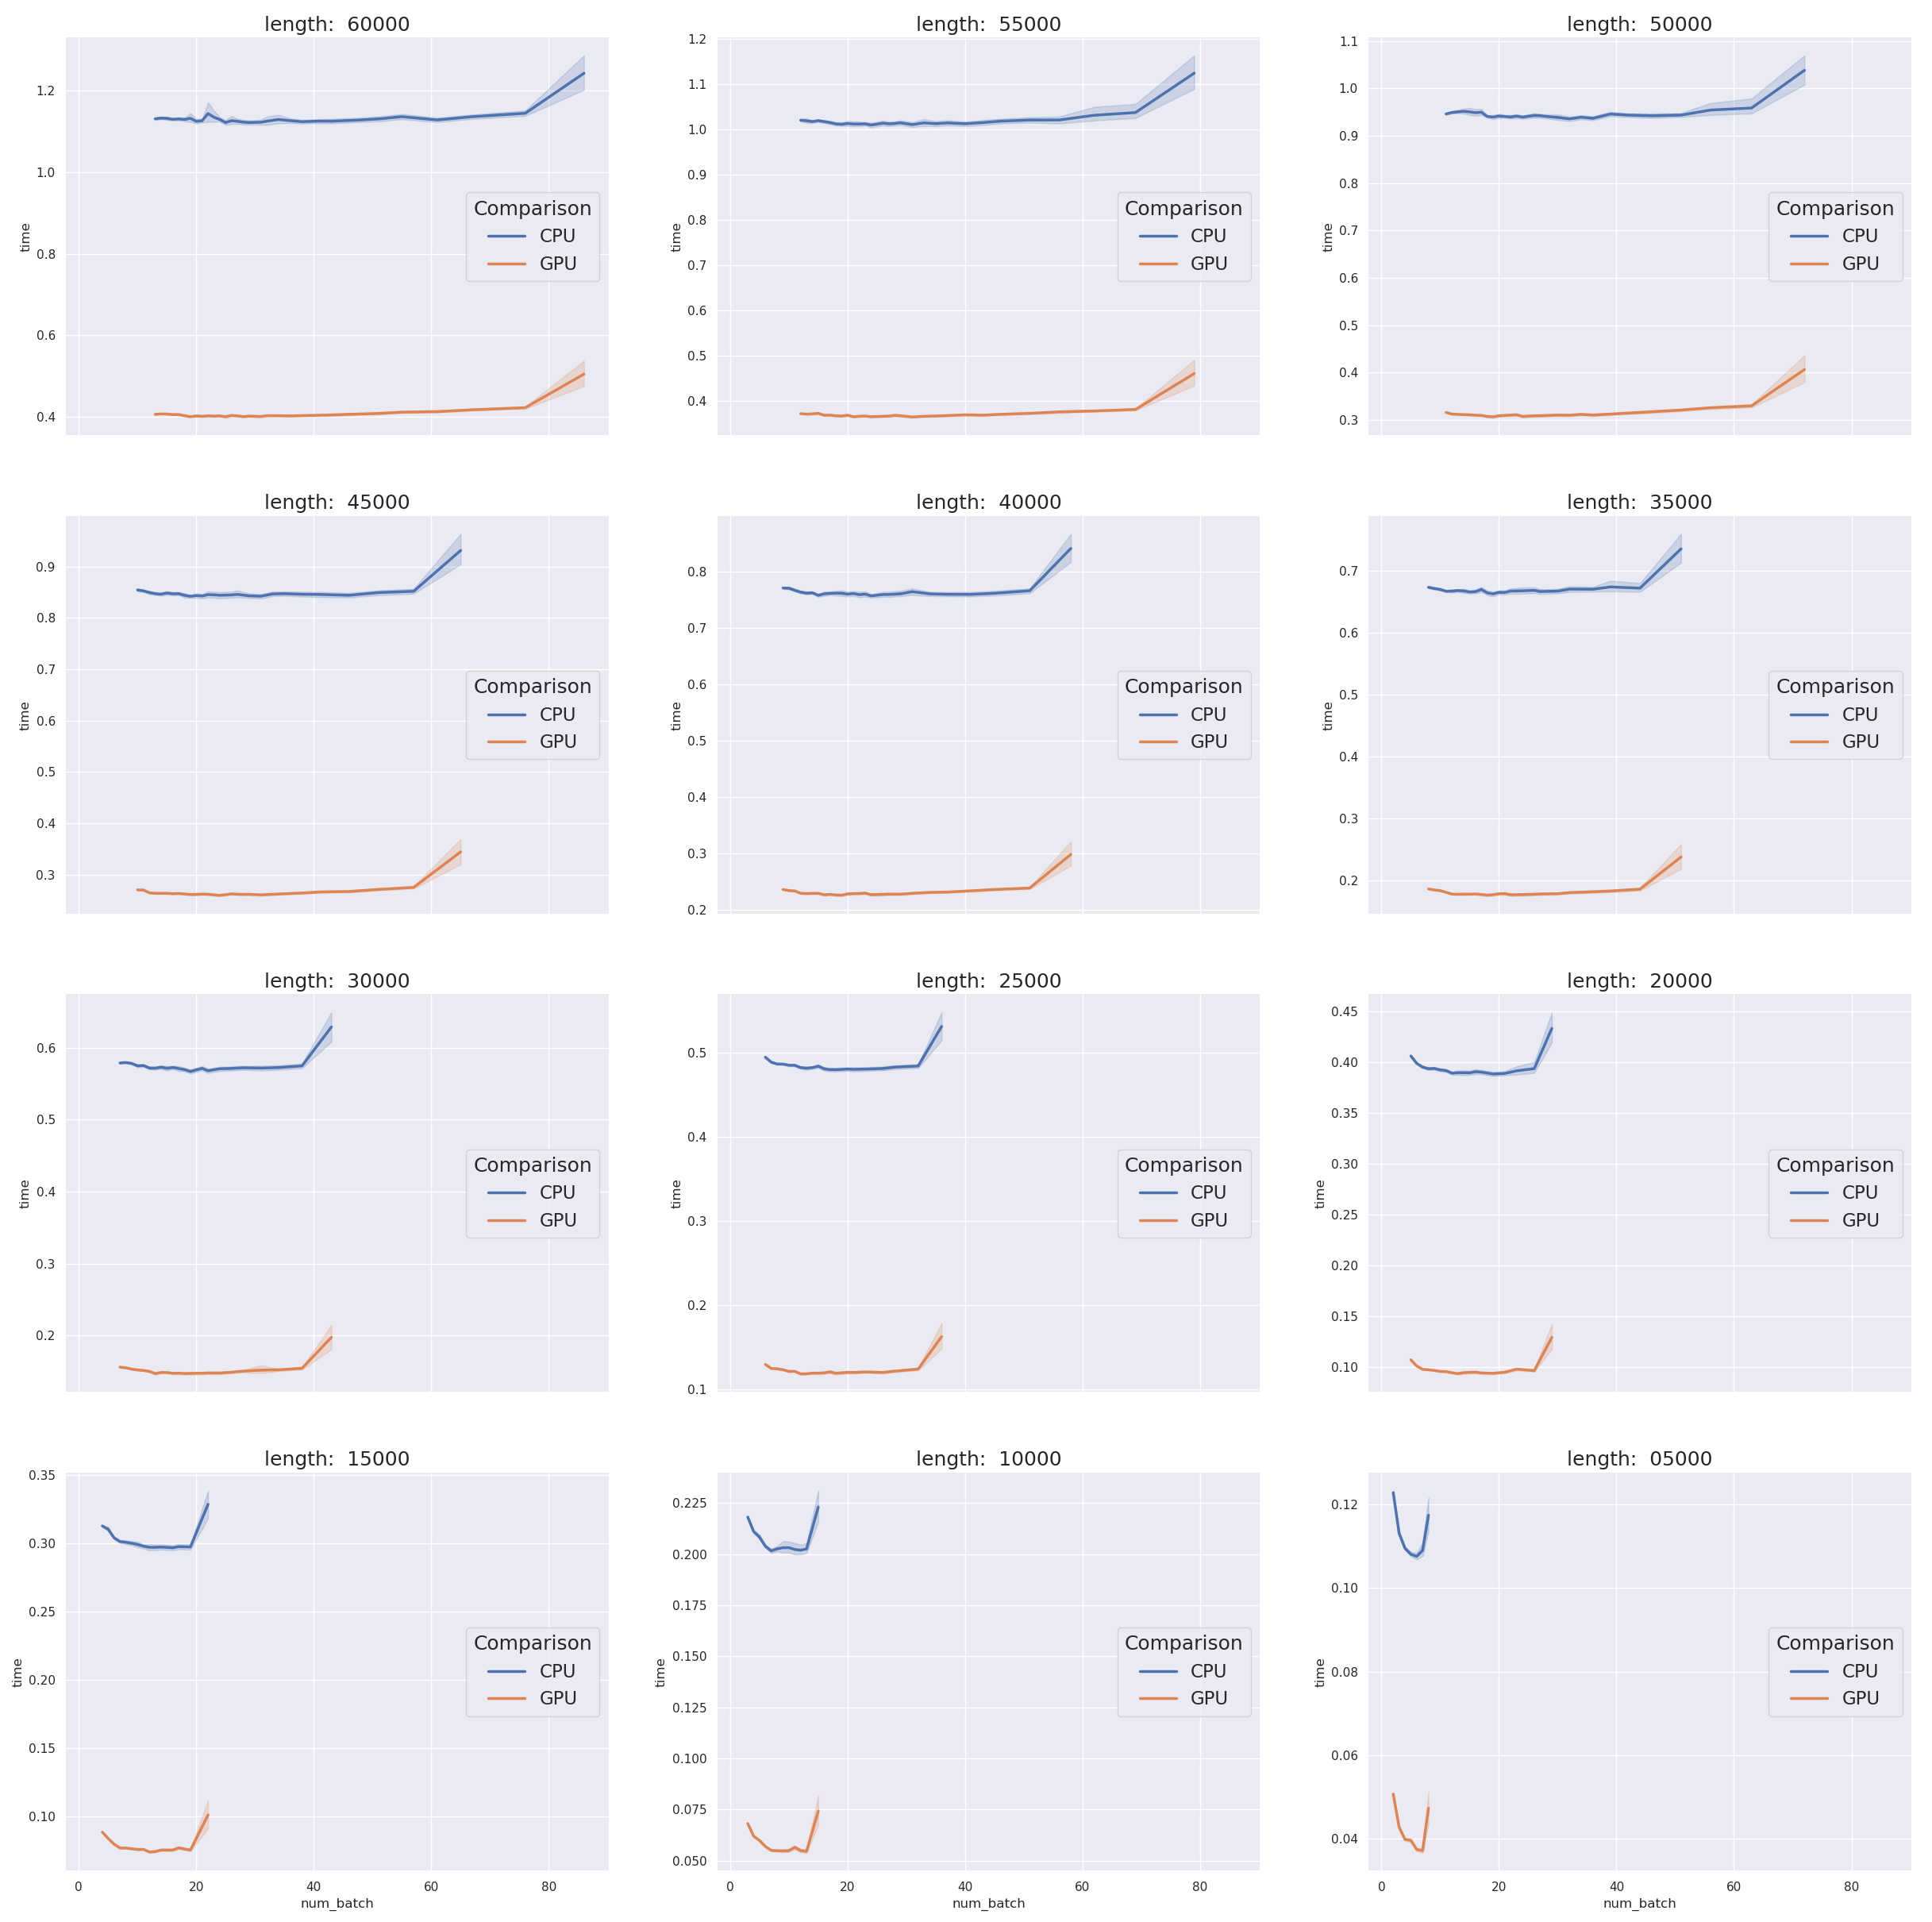
\includegraphics[width=\textwidth]{img/num_CPU_vs_GPU_Grid}
\caption{\label{fig:num_CPU_vs_GPU_Grid.}Зависимость времени работы от количества пакетов}
\end{figure}

\newpage
\section*{Оформить как приложение 3}
\label{sec:code}
\addcontentsline{toc}{section}{\nameref{sec:code}}

\begin{ListingEnv}[h]
\begin{lstlisting}
def flexible_batch_indices(text, approximate_batch_size):
    exp = r'[.?!](?= [A-Z]|$)'
    cur_index = 0
    find_start = 0
    batch_indices = [0]
    sentence_found = False
    # Continue while start index < text length.
    while find_start < len(text):
        find_start = cur_index + approximate_batch_size
        find_end = find_start + approximate_batch_size

        # Check if the right index is less or equal to the length of the text.
        if find_end > len(text):
            find_end = len(text)
     
        match = re.search(exp, text[find_start:find_end])
        # If a match is found, recalculate the indices and add to the list.
        if match:
            cur_index = match.end() + find_start - 1
            batch_indices.append(cur_index)
            sentence_found = True
        else:
            # Just shift the index otherwise.
            cur_index += approximate_batch_size
            sentence_found = False
    if sentence_found:
        batch_indices.append(len(text))
        
    return batch_indices
\end{lstlisting}
\caption{Обработка \emph{'aux'} при поиске конструкций \emph{Passive Voice}}
% далее метка для ссылки:
\label{list:aux}
\end{ListingEnv}




%
%%
%%
%\newpage
%\subsection{Как вставлять листинги и рисунки}
%
%Для крупных листингов есть два способа. Первый красивый, но в нём не допускается
%кириллица (у вас может встречаться в комментариях и
%печатаемых сообщениях), он представлен на листинге~\ref{list:hwbeauty}.
%\begin{ListingEnv}[t]
%\begin{lstlisting}
%
%getStrippedBody: function (html) {
%  let body = html.match(/<body[^>]*>(?:([^]*)<\/body>([^]*)|([^]*))/i);
%  if (body && body.length > 1) {
%  if (body[2] && body[2].length > this.minBodyTailLength()) {
%        body = body[1] + ' ' + body[2];
%      } else if (body[1] === undefined) {
%                body = body[3];
%            } else {
%                body = body[1];
%            }
%        } else {
%            body = html;
%        }
%
%        return body.replace(/<script\b[^>]*(?:>[^]*?<\/script>|\/>)/ig, '<blink/>');
%    },
%\end{lstlisting}
%\caption{Программа “Hello, world” на \protect\cpp}
%% далее метка для ссылки:
%\label{list:hwbeauty}
%\end{ListingEnv}

%Второй не такой красивый, но без ограничений (см.~листинг~\ref{list:hwplain}).
%\begin{ListingEnv}[H]
%\begin{Verb}
%
%#include <iostream>
%using namespace std;
%
%int main()
%{
%    cout << "Привет, мир" << endl;
%}
%\end{Verb}
%\caption{Программа “Hello, world” без подсветки}
%\label{list:hwplain}
%\end{ListingEnv}
%
%Можно использовать первый для вставки небольших фрагментов
%внутри текста, а второй для вставки полного
%кода в приложении, если таковое имеется.
%%
%%Если нужно вставить совсем короткий пример кода (одна или две строки), то выделение  линейками и нумерация может смотреться чересчур громоздко. В таких случаях можно использовать окружения \texttt{lstlisting} или \texttt{Verb} без \texttt{ListingEnv}. Приведём такой пример с указанием языка программирования, отличного от заданного по умолчанию:
%\begin{lstlisting}[language=Haskell]
%fibs = 0 : 1 : zipWith (+) fibs (tail fibs)
%\end{lstlisting}
%Такое решение~--- со вставкой нумерованных листингов покрупнее
%и вставок без выделения для маленьких фрагментов~--- выбрано,
%например, в книге Эндрю Таненбаума и Тодда Остина по архитектуре
%компьютера~\autocite{TanAus2013} (см.~рис.~\ref{fig:tan-aus}).
%
%Наконец, для оформления идентификаторов внутри строк
%(функция \lstinline{main} и тому подобное) используется
%\texttt{lstinline} или, самое простое, моноширинный текст
%(\texttt{\textbackslash texttt}).
%
%\begin{figure}[p]% p означает, что нужно выделить для рисунка
%% отдельную страницу; применяется для больших рисунков
%\centering
%%Здесь могла быть ваша лягушка.
%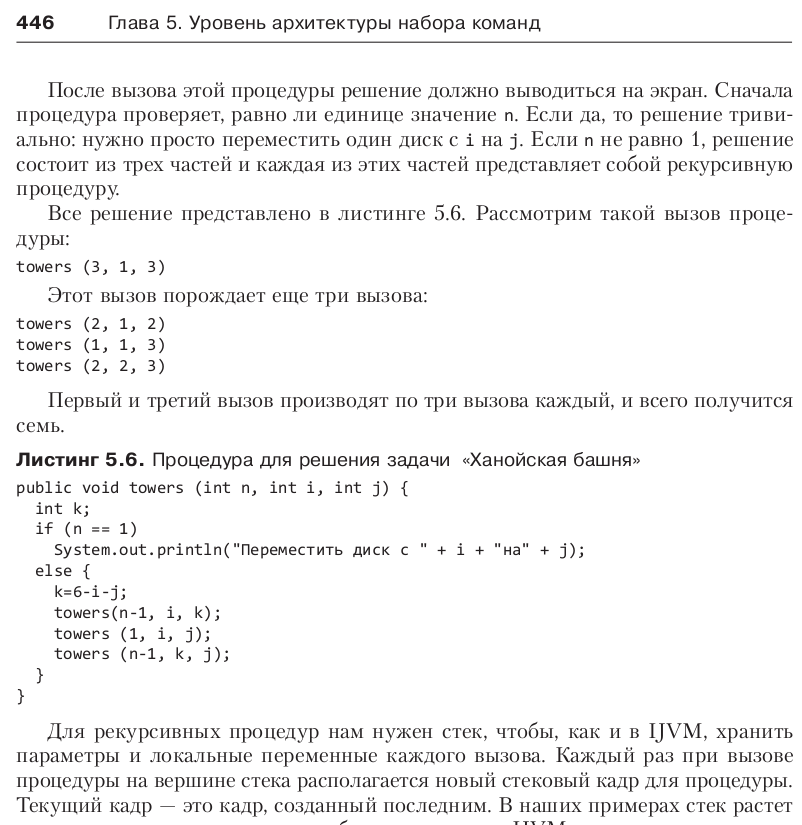
\includegraphics[width=\textwidth]{img/tan-aus.png}
%\caption{\label{fig:tan-aus}Пример оформления листингов в~\autocite{TanAus2013}}
%\end{figure}
%
%Использовать внешние файлы (например, рисунки) можно и на \href{http://overleaf.com}{overleaf.com}: ищите кнопочку upload.
%
%\subsection{Как оформить таблицу}
%
%Для таблиц обычно используются окружения table и tabular --- см. таблицу~\ref{tab:widgets}. Внутри окружения tabular используются специальные команды пакета booktabs — они очень красивые; самое главное: использование вертикальных линеек считается моветоном.
%
%\begin{table}
%\centering
%\caption{\label{tab:widgets}Подпись к таблице --- сверху}
%\begin{tabular}{llr}
%\toprule
%\multicolumn{2}{c}{Item} \\
%\cmidrule(r){1-2}
%Животное  & Описание    & Цена (\$) \\
%\midrule
%Gnat      & per gram    & 13.65      \\
%          & each        & 0.01       \\
%Gnu       & stuffed     & 92.50      \\
%Emu       & stuffed     & 33.33      \\
%Armadillo & frozen      & 8.99       \\
%\bottomrule
%\end{tabular}
%\end{table}
%
%\subsection{Как набирать формулы}
%
%\LaTeX{} is great at typesetting mathematics. Let $X_1, X_2, \ldots, X_n$ be a sequence of independent and identically distributed random variables with $\text{E}[X_i] = \mu$ and $\text{Var}[X_i] = \sigma^2 < \infty$, and let
%$$S_n = \frac{X_1 + X_2 + \cdots + X_n}{n}
%      = \frac{1}{n}\sum_{i}^{n} X_i$$
%denote their mean. Then as $n$ approaches infinity, the random variables $\sqrt{n}(S_n - \mu)$ converge in distribution to a normal $\mathcal{N}(0, \sigma^2)$.
%
%\subsection{Как оформлять списки}
%
%Нумерованные списки (окружение enumerate, команды item)…
%
%\begin{enumerate}
%  \item Like this,
%  \item and like this.
%\end{enumerate}
%
%\dots маркированные списки \dots
%
%\begin{itemize}
%  \item Like this,
%  \item and like this.
%\end{itemize}
%
%\dots списки-описания \dots
%
%\begin{description}
%  \item[Word] Definition
%  \item[Concept] Explanation
%  \item[Idea] Text
%\end{description}
%
%\Conc
%
%Помните, что на все пункты списка литературы должны быть ссылки. \LaTeX\ просто не добавит информацию об издании из bib"/файла, если на это издание нет ссылки в тексте. Часто студенты используют в работе  электронные ресурсы: в этом нет ничего зазорного при одном условии: при каждом заимствовании следует ставить соответствующую ссылку. В качестве примера приведём ссылку на сайт нашего института~\autocite{mmcs}.
%
%Для дальнейшего изучения \LaTeX\ рекомендуем книгу Львовского~\autocite{Lvo2003}: она хорошо написана, хотя и несколько устарела.
%Обычно стоит искать подсказки на
%\href{http://tex.stackexchange.com/}{tex.stackexchange.com}, а также
%читать документацию по установленным пакетам с помощью
%команды
%\begin{Verb}
%texdoc имя_пакета
%\end{Verb}
%или на \href{http://ctan.org/}{ctan.org}.

%% Печать списка литературы (библиографии)
%\newpage
%
%\printbibliography[%{}
%    heading=bibintoc%
%    %,title=Библиография % если хочется это слово
%]
% Файл со списком литературы: biblio.bib
% Подробно по оформлению библиографии:
% см. документацию к пакету biblatex-gost
% http://ctan.mirrorcatalogs.com/macros/latex/exptl/biblatex-contrib/biblatex-gost/doc/biblatex-gost.pdf
% и огромное количество примеров там же:
% http://mirror.macomnet.net/pub/CTAN/macros/latex/contrib/biblatex-contrib/biblatex-gost/doc/biblatex-gost-examples.pdf

\end{document}
